\chapter{Machine Learning and Latent Space Equilibrium}
%
\begin{quote}
"It is widely believed that the real-world data is generated by a few explanatory factors which are distributed, invariant and disentangled" (Bengio et al., 2013).
\end{quote}
%
As previously described in the introductory chapter we are being spectators in this decade of a deep advance in the computation technology that opened for data-science the era of \textit{big data}. There are millions of autonomous software components that continuously crawl the internet network decoding HTML pages from 60 billion of pages collected and indexed in a single database. Each time we capture a picture this file is automatically classified and stored in a cloud space that is claimed to receive 1.2 billion of pictures per day. 
%
We can define ML as the available set of tools that analyzing such big amount of information are automatically providing a possible uncovered pattern among them to be eventually able to predict a future output of the system and operate any other kind of decision based on data uncertainty. The intimate meaning of \textit{machine learning} in this context is referred to the fact that the human intervention is on the very base of the algorithm structural definition while it is the actual model itself that stitches to the input data.  

In science, there are essentially two modelling approaches: \textbf{data driven models}; and \textbf{process based models}.
Although physical modeling is the main primary tool to understand the behaviour of natural processes, and to make inference about the future outcomes, it is becoming an increasingly exploited solution to employ a data driven approach where the process based physical models appear to be not detailed enough to describe complex systems in operational situations. For instance we often look at the sole main physical phenomenon where the output measured quantities are actually corrupted by non linear cascade of underlying effects, or we are even looking at an unknown behavior for which the model results to be a partial or even a wrong description for the actual measured representation. 
In some other cases an hybrid version of combined physical and statistical model could be also explored, as we will see in the next sections. But the actual point is that we start to look at the measures of an experiment, not only from the perspective of the single independent experience but from a more general point of view that takes into account the whole repetition history and a wider operational space.  


\section{Statistical description of DNN}

As already anticipated, in order to gather the wide range of all the possible concurring physical causes that drive the measures, we decided to make use of the latest novel approach of Deep Neural Networks. As a preliminary backward step, this section would provide a slight general description that bases this approach in a statistical oriented fashion; this is the preferred mathematical representation of the recurrent/repeatable output of a scientific experiment lead by the probability theory as it was generalized by Pierre Laplace (1812). 

The collated set of all measures along the consecutive experimental repetitions is often referred as the model \textit{dataset}, while a single instance of this dataset with a proper selection of the quantities under analysis is commonly called \textit{features} or \textit{covariates}\footnote{The most precise definition seems to be the term covariate used in Analysis of Covariance, a type of General Linear Model in which the independent variables of interest are categorical, but you also need to adjust for the effect of an observed, continuous variable–the covariate}.
%
If we consider our dataset in the generic physical model outputs we can refer as the single input feature of the ML model as a stochastic vector $\bm{x} = [x_1,x_2, ... ,x_N]$ that is characterized by its probability density distribution $p(\bm{x})$. The very general macroscopic description of any machine learning application consists to feed a statistical model with this input feature eventually providing as output the \textit{p.d.f} of another related measure $p(y|\bm{x})$ or a description of $p(\bm{x})$ itself. These two kinds of results are respectively representative of the so called  \textbf{supervised} and \textbf{unsupervised} learning: in the former the the model is confronted with a known relation between variables, while any information is provided to the model for the latter but we are simply looking at the distribution of the variables in their own manifold or in a subspace (as it will described in the next sections).

The unitary element that composes either the standard \textit{Neural Network} structure and the \textit{Deep Neural Network} is the so called \textit{Single Layer Perceptron}; in the following it will be shown that this particular element can be seen as a single instance of a \ac{GLM}, while the operation performed by each of this quantity is a generic regression model applied on its input features.
%
Although GLM is the generalized representation of the ordinary linear regression we shall first introduce the latter as a first example to present the formalism in a simpler manner.
The very basic linear regression model is a linear mapping from N-dimensional input features (or covariates) $\bm{x}$, to a set of targets (or responses) $\bm{y}$, using the inputs, a set of weights (or regression coefficients) $\bm{w}$ and a bias offset $w_0$. The internal product of features and weights gives the equation of the fitter that in the linear form has the shape of a line in the N-dimensional space. The line is centered within the input data while typically the probabilistic model assumes that the residuals can be described with a Gaussian shape of unknown variance $\sigma^2$. The model can be written as a predictor in the form:
\begin{equation}
    \hat{y} = \eta + \epsilon
\end{equation}
where
\begin{equation}
     \eta = \transpose{\bm{w}}\bm{x} \qquad  \epsilon \in \mathcal{N}(0,\sigma^2)
\end{equation}
the first addendum is the \textit{linear predictor} in which a scalar is appended at the end of the the weight vector to fit the bias of the distribution, and the second addendum represents the overall error. To let the model fitting also the bias the parameters and covariates array have been rewritten as follows:
\begin{equation}
    \bm{w} = [\hat{\bm{w}},w_0] \qquad \bm{x} = [\hat{x}, 1]
\end{equation}
At this point the conditional probability of the target given the features can be modeled as a Gaussian distribution:
\begin{equation}
    p(y|\bm{x}) = \mathcal{N}(\eta, \sigma^2)
\end{equation}
this happens because we forced to consider the features with normal distribution and because being an exponential distribution it is also a conjugate prior for the likelihood, as it will described in the following.


%   ____ _     __  __ 
%  / ___| |   |  \/  |
% | |  _| |   | |\/| |
% | |_| | |___| |  | |
%  \____|_____|_|  |_|
%
\subsection{Generalized Linear Models}
The use of exponential distribution turns to be a very clever solution. Indeed, among all families of distributions, where the definition domain does not vary with the parameter being estimated, this family is the only one with a sufficient statistic whose dimension remains bounded if the sample size increases. This means that we can have a compressed representation of the dataset into a fixed size summary without loss of information.
Exponential families are also important in Bayesian reconstruction where a prior distribution is multiplied by a likelihood function and normalized to produce the posterior. In the case of a likelihood which belongs to an exponential family there always exists a conjugate prior, which is usually also exponentially distributed. 
%
%A conjugate prior for the parameter $\eta$ of an exponential family
The formal definition of a generic exponentially distributed p.d.f. is the following:
%% EXPONENTIAL
\begin{equation}
    p(x|\theta) = \frac{1}{Z(\bm{\theta})}h(x) \exp{[\transpose{\bm{\theta}} \phi(\bm{x})]}
\end{equation}
where $\bm{\theta} \in \Theta \subseteq \mathbb{R}^d$ are defined as the \textbf{natural parameters}, $\phi(\bm{x}) \in \mathbb{R}^d$ is called the vector of \textbf{sufficient statistics}, $h(\bm{x})$ is a scaling factor that is usually a unitary constant, and $Z(\bm{\theta})$ is the \textbf{partition function} that normalizes the distribution:
\begin{equation}
    Z(\bm{\theta}) = 
    \int_{\mathcal{X}^n} h(\bm{x}) \exp{[\transpose{\bm{\theta}} \phi(\bm{x})]} dx
\end{equation}
Being all the arguments within an exponential operator it is also quite common to embed the partition function too, using $ A(\bm{\theta}) = \log\left(Z(\bm{\theta})\right)$ in the following:
\begin{equation}
    p(x|\bm{\theta}) = h(\bm{x}) \exp{[\transpose{\bm{\eta}}\phi(\bm{x}) - A(\bm{\eta}) ]}
\end{equation}
where the function $\eta$ has been further introduced to expand the natural parameters to the representation $\bm{\eta}=\eta(\bm{\theta})$, where $\text{dim}(\bm{\theta}) \leq \text{dim}\left(\eta(\bm{\theta})\right)$.

%% BERNOULLI EXPONENTIAL
\subsubsection*{example: exponential representation of the Bernoulli distribution}
The Bernoulli distribution for $x\in\{0,1\}$ can be written in exponential family form as:
\begin{equation}
\begin{split}
    \text{Ber}(x|\mu) &= \mu^x(1-\mu)^{1-x} \\
%                      &= (1-\mu) \exp{\left[ x \log\left(\frac{\mu}{1-\mu}\right)\right]} \\
                      &= \exp{\left[\transpose{\phi(x)}\bm{\theta} \right]}
\end{split}
\end{equation}
where we set:
\begin{align*}
  & \phi(x) = x \\
  & \theta  = \log\left(\frac{\mu}{1-\mu}\right) \\
  & Z = 1/(1-\mu)
\end{align*}

%% GAUSSIAN EXPONENTIAL
\subsubsection*{example: exponential representation of the Univariate Gaussian distribution}
The univariate Gaussian can be written in exponential family in this form:
\begin{equation}
\begin{split}
        \mathcal{N}(x|\mu,\sigma^2) &= \frac{1}{(2\pi\sigma^2)^\frac{1}{2}} \exp{\left[-\frac{1}{2\sigma^2}(x-\mu)^2\right]} \\
        & \frac{1}{Z(\bm{\theta}}\exp{\left[\transpose{\bm{\theta}}\bm{\phi}(x)\right]}
\end{split}
\end{equation}
once the parameters have been set to:
\begin{align*}
    & \bm{\phi}(x) = \left[ x, x^2 \right] \\
    & \bm{\theta}  = \left[ \frac{\mu}{\sigma^2}, -\frac{1}{2\sigma^2} \right] \\
    & Z(\mu,\sigma^2) = \sqrt{{2\pi\sigma^2}} \exp{\left[ \frac{\mu^2}{2\sigma^2} \right]}
\end{align*}

%%GLM
It has been shown that the linear regression predicts the expected value of a given quantity as a linear combination the dataset. This implies that a constant change in the covariates leads also to a constant change in the response (i.e. a linear-response model). This is appropriate when the response variable has a normal distribution (intuitively, when a response variable can vary essentially indefinitely in either direction with no fixed "zero value", or more generally for any quantity that only varies by a relatively small amount).
However, these assumptions are inappropriate where the response variable is expected to have a different shape. 
% RR
As an example, a prediction model might predict that 10 degree temperature decrease would lead to 1,000 fewer people visiting the beach is unlikely to generalize well over both small beaches (e.g. those where the expected attendance was 50 at a particular temperature) and large beaches (e.g. those where the expected attendance was 10,000 at a low temperature). The problem with this kind of prediction model would imply a temperature drop of 10 degrees would lead to 1,000 fewer people visiting the beach, a beach whose expected attendance was 50 at a higher temperature would now be predicted to have the impossible attendance value of -950. Logically, a more realistic model would instead predict a constant rate of increased beach attendance (e.g. an increase in 10 degrees leads to a doubling in beach attendance, and a drop in 10 degrees leads to a halving in attendance). Such a model is termed an exponential-response model (or log-linear model, since the logarithm of the response is predicted to vary linearly).
%% 
Generalized linear models overcome this limitation extending the ordinary linear models expanding the response variables to any arbitrary distribution (rather than simply the normal), imposing an arbitrary function of the response variable (the link function) to exploit the linearity with the predicted values. 
% RR
For example, the case above of predicted number of beach attendees would typically be modeled with a Poisson distribution and a log link, while the case of predicted probability of beach attendance would typically be modeled with a Bernoulli distribution (or binomial distribution, depending on exactly how the problem is phrased) and a log-odds (or logit) link function.
%%GLM
The three main ingredients of a GLM are:
\begin{itemize}
    \item The \textbf{exponential family} of probability distributions,
    \item the usual \textbf{linear predictor} $\eta = \transpose{\bm{w}}\bm{x}$,
    \item a \textbf{link function} $g$ such that $\expectation{y|\bm{x}} = \mu = g^{-1}(\eta)$.
\end{itemize}

The GLM probability is composed as follows:
\begin{equation}
    p(y_i| \theta, \sigma^2) = 
    \exp{\left[ \frac{y_i\theta - A(\theta}{\sigma^2} + c(y_i,\sigma^2) \right] }
\end{equation}


%
%  _____ ___ _     _       _   _ _____ ____  _____ 
% |  ___|_ _| |   | |     | | | | ____|  _ \| ____|
% | |_   | || |   | |     | |_| |  _| | |_) |  _|  
% |  _|  | || |___| |___  |  _  | |___|  _ <| |___ 
% |_|   |___|_____|_____| |_| |_|_____|_| \_\_____|
%

%% GLM

%% GAUSSIAN MODEL EXAMPLE

%% CLOSED FORM FOR GAUSSIAN MODEL


%   ____                 _     _           _ __  __           _      _     
%  / ___|_ __ __ _ _ __ | |__ (_) ___ __ _| |  \/  | ___   __| | ___| |___ 
% | |  _| '__/ _` | '_ \| '_ \| |/ __/ _` | | |\/| |/ _ \ / _` |/ _ \ / __|
% | |_| | | | (_| | |_) | | | | | (_| (_| | | |  | | (_) | (_| |  __/ \__ \
%  \____|_|  \__,_| .__/|_| |_|_|\___\__,_|_|_|  |_|\___/ \__,_|\___|_|___/
%                 |_|       
%
\subsection{Directed Graphical Models}
In the previous chapter we saw a possible general approach to obtain a regression of a single target variable given its conditional probability with an input process. Suppose now that we are observing a set of multiple correlated variables where the correlation extends from one variable to another in a chain of dependencies. This becomes a stochastic model describing a sequence of possible values for the variables in which the probability of each event depends on the state of the others.
If we constrain the variable correlation to be strictly ordered the probability of a target variable after all the correlation hops can be written as:
\begin{equation}
    p(x_1, x_2, ... x_V | \bm{\theta}) = p(x_1|\bm{\theta})p(x_2|x_1,\bm{\theta})p(x_3|x_2,x_1,\bm{\theta}) ... p(x_V|x_1, ... x_{V-1},\bm{\theta})
\end{equation}
Looking at all the possible $p(x_i|\bm{\theta})$ the conditional links among variable appears as a linked directed graph.
%
This is called “Graphical model” as it combines graph theory and probability theory to provide a general framework to represent variables interaction. Graphical models trace their origins to many different fields and have been applied in wide variety of settings: for example, to develop probabilistic expert systems, and to understand neural networks. Remarkably, the very same formalism and algorithms can be applied to a wide range of problems.
%
However even if the pictorial result is quite intuitive, the joint relation among stochastic variables can easily grow exponentially; for instance if we imagine all distributions having the same finite discrete support composed by $K$ states the representation of all $p(x_i|x_j)$ is $O(K^2)$, the representation of $p(x_i|x_j,x_k)$ is $O(K^3)$ and so forth, so the overall model of V cardinality would become $O(K^V)$. This description of joint discrete possible states, known as the \textbf{conditional probability table}, is sometimes used to describe a fully observed covariates vector in the complete statistical description of the complex systems of variable. Actually this solution, beside requiring a first restriction in the number of possible states that represents each stochastic process, it is also presenting a critical convergence requiring a awful amount of data to reach a meaningful state for such amount of parameters.
One possible solution, in the same discrete approximation, is to make use a more compact conditional distribution function, such as the multinomial logistic i.e. $p(x_i | \bm{x_j})_{i \neq j} = S_k(\bm{W}_i \bm{x_{j}}$). Although this model has been successfully applied in literature for some generative classifiers~\cite{Bengio:1999:MHD:3009657.3009714}, it appears to remain an overkill in conditioning the system.

Another practical end very common solution is to assume a conditional Independence among variables that are k-hops distant from the others, exploiting the \textbf{Markov assumption} of independence among the link graph.
For example, under these conditions, imposing a single hop Independence, the chains of links that create are constituted by first order \textbf{Markov chain} shown in the first diagram of \Figure{\ref{fig:simple_markov_chains_a}}, and described by the following joint distribution:
\begin{equation}
    p(x_1, x_2, ... x_V) = p(x_1) \prod_{j=1}^V p(x_j|x_{j-1})
\end{equation}
equivalently the second order independence can be imposed, generating a graph like in \Figure{\ref{fig:simple_markov_chains_b}} describe by:
\begin{equation}
    p(x_1, x_2, ... x_V) = p(x_1) \prod_{j=1}^V p(x_j|x_{j-1},x_{j-2})
\end{equation}
In the same way higher-order Markov models can be created, however even the second-order Markov assumption may be inadequate if there are long-range correlations throughout the available observations since the number of parameters will again blow up. 





\begin{figure}
    \centering
    \subfigure[]{
    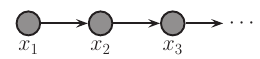
\includegraphics[width=0.3\textwidth]{img/3_ML/DGM_o1_markov.png}
    \label{fig:simple_markov_chains_a} }
    \subfigure[]{
    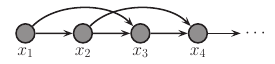
\includegraphics[width=0.3\textwidth]{img/3_ML/DGM_o2_markov.png}
    \label{fig:simple_markov_chains_b} }
    \caption{First order (a) and second order (b) Markov Chain examples, the arrow represents a conditional probability that relates variables each other.}
    \label{fig:simple_markov_chains}
\end{figure}

\begin{figure}
    \centering
    \subfigure[]{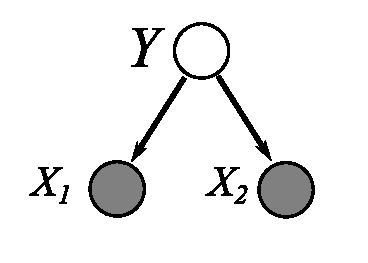
\includegraphics[height=2cm]{img/3_ML/naive_bayes_1.pdf}
    \label{fig:naive_bayes}}
    \subfigure[]{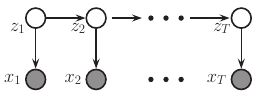
\includegraphics[height=2cm]{img/3_ML/DGM_o1_hmm.png}
    \label{fig:hidden_markov}}
    \caption{Caption}
\end{figure}

A further possible reduction in the number of joint relations between observed variables can be also given by the formalism itself,  by the assumption that some covariates are correlated because they all arise from a hidden common “cause”. Those common causes can be described as variables themselves but that can't be directly accessed.  Model with hidden variables are also known as latent variable models or LVMs. 
The very basic example i the \textbf{naive Bayes classifier}, where features are assumed to be conditionally independent given a class label a common target. This is illustrated in \Figure{\ref{fig:naive_bayes}}. The joint probability can be then written as:
\begin{equation}
    p(y,\bm{x}) = p(y) \prod_{j=1}^V p(x_j| y)
\end{equation}
%
Another very powerful alternative approach is to assume that there is an underlying hidden process, that can be modeled by a first-order Markov chain, but for which available measures is a noisy observation of this process. The result is known as \acl{HMM}, shown in \Figure{\ref{fig:hidden_markov}}. 




\begin{figure}
    \centering
    \subfigure{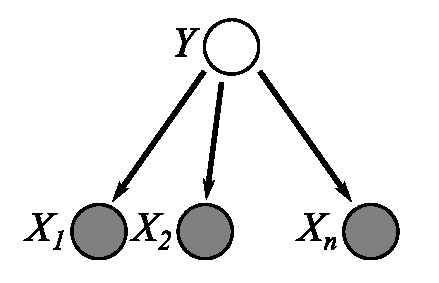
\includegraphics[height=2.5cm]{img/3_ML/naive_bayes_2.pdf} \label{fig:plate_naive_bayes}}
    \subfigure{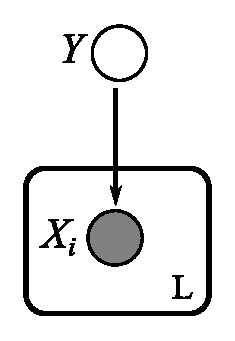
\includegraphics[height=2.5cm]{img/3_ML/plate_ntz_1.pdf} \label{fig:plate_ntz_1}}
    \subfigure{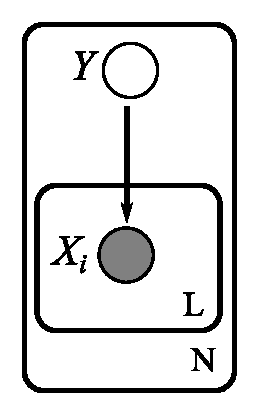
\includegraphics[height=2.5cm]{img/3_ML/plate_ntz_2.pdf} \label{fig:plate_ntz_2}}
    \caption{ Plate notation for DGM }
    \label{fig:plate_notation}
\end{figure}






%  _____ _____ ____  _   _      _                      _    
% |  ___|  ___|  _ \| \ | | ___| |___      _____  _ __| | __
% | |_  | |_  | | | |  \| |/ _ \ __\ \ /\ / / _ \| '__| |/ /
% |  _| |  _| | |_| | |\  |  __/ |_ \ V  V / (_) | |  |   < 
% |_|   |_|   |____/|_| \_|\___|\__| \_/\_/ \___/|_|  |_|\_\
%
\subsection{Feed forward dense network}
\label{section:feedforward dense networks}
%
A feed forward NN, aka \ac{MLP} is again using the linear regression, actually it can be seen as a chain of logistic regression models that are stacked one on top of each other, where the final layer being a \ac{GLM}, either a logistic or a linear regression depending weather we are looking for a general classification output (i.e. a probability function output for each of the classes in the classifier domain) or a regression output. 
For instance, looking at the simple two layers example, and considering a regression output problem, the model would be written like:
\begin{equation}
    p(y|\bm{x},\bm{\theta}) = \mathcal{N}\left(y|\transpose{\bm{w}}\bm{z(\bm{x}}), \sigma^2 \right)
    \label{eq:mlp_a}
\end{equation}
where the basis function expansion here is a non-linear response of further linear combination of the inputs:
\begin{equation}
    \bm{z}(\bm{x}) = \left[ g(\transpose{\bm{v}_1}\bm{x}), g(\transpose{\bm{v}_2}\bm{x}), ..., g(\transpose{\bm{v}_H}\bm{x})
    \right]
    \label{eq:mlp_b}
\end{equation}
the transformation $z(\bm{x})$ represents here the non-linear transformation on regression in which the deterministic function $g(\bm{x},\bm{v})$, also called the \textbf{activation function}, is the kernel of the basis function expansion. In this way we could think of the \acl{MLP} as a kernel machine where the kernel functions have been opportunely shaped to match the input data. This parametrization on the kernel function makes the \acl{MLP} an \ac{ABM}:
\begin{equation}
    f(\bm{x}) = \transpose{\bm{w}}\bm{\phi}(\{1,\bm{x}\}, \bm{V})
\end{equation}
The generic basis function $\phi(\bm{x},\bm{V})$ must be trained on the dataset to make it "adapt" at the input statistics; while
the entire parameter set that embrace the kernel is now: $\bm{\theta} = (\bm{w}, \bm{v})$ with $\bm{w} = [w_0, w_1, ..., w_M]$ and $\bm{v}_m = [v_{m1}, v_{m2}, ..., v_{mH}]$. The first set of parameters are the linear combination coefficients of the \ac{GLM}, and the second are the parametrization of the kernel. The unit appended to the input feature has been used to add the bias coefficient $w_0$.

\begin{figure}
    \centering
    \subfigure[]{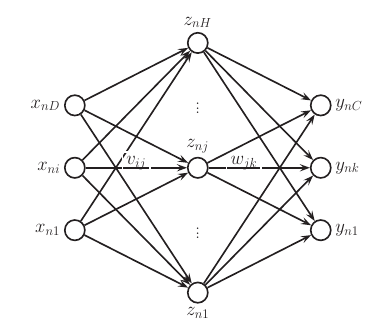
\includegraphics[height=4cm]{img/3_ML/MLP.png} \label{fig:mlp_a}}
    \subfigure[]{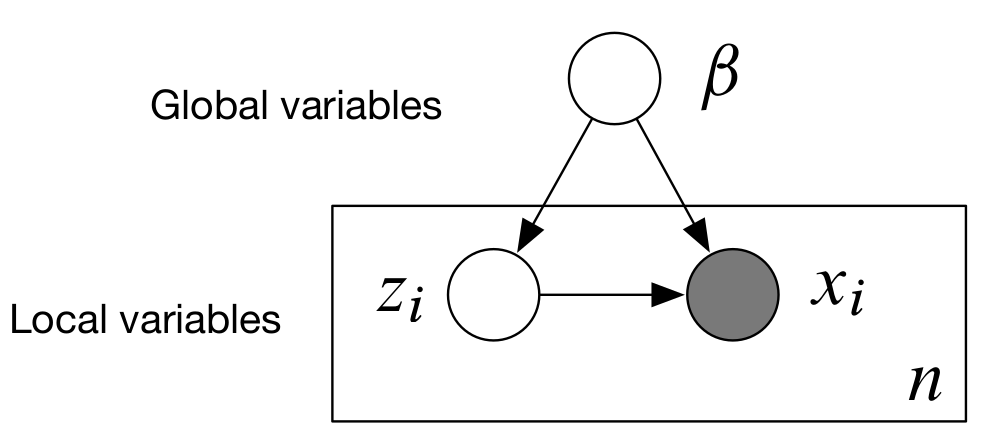
\includegraphics[height=4cm]{img/3_ML/FDN_plate_model.png}}
    \caption{One hidden layer Feed Forward Neural Network (or equivalently the minimal Multi Layer Perceptron, seen as an Adaptive Basis Function Model (a), and the equivalent model in plate notation (b). }
    \label{fig:mlp}
\end{figure}

The final \acl{GLM} applied can be constructed as usual in many different shapes, depending on the target type of inference we are interested in. If we look for a binary classification it appears as a logistic regression, i.e. the fit on the Bernoulli distribution of the sigmoid outputs:
\begin{equation}
    p(y|\bm{x}, \bm{\theta}) = \text{Ber}\left( y|\text{sigm}(\transpose{\bm{w}}\bm{z}(\bm{x}) \right)
\end{equation}
If we are looking for categorical classifier the correct GLM has to be distributed as:
\begin{equation}
    p(y|\bm{x}, \bm{\theta}) = \text{Cat}\left( y|\mathcal{S}(\transpose{\bm{w}}\bm{z}(\bm{x})) \right)
\end{equation}
where the \textit{Cat} distribution is the Multinulli and $\mathcal{S}$ stands for the support function of the input.
Finally as stated in the first example if we are fitting a generic output function it will appear for example as a Gaussian regression model:
\begin{equation}
    p(\bm{y}|\bm{x}, \bm{\theta}) = \mathcal{N}\left( \bm{y}|\bm{W} \phi \right)
\end{equation}
where in this last version of the formula the probability has been shaped with the weights matrix $\bm{W}$ taking into account the possible MIMO configuration of the perceprton as shown in \Figure{\ref{fig:mlp_a}}.
It is finally a key factor for the activation function $g(\bm{x},\bm{v})$ to be a non-linear operator because the overall network would collapse into a large linear regression otherwise. Usually the activation is the logistic function $g(u) = \text{sigm}(u)$ or the recently much common flavors of the \textbf{rectified linear units} (ReLU) that provide a non linear activation with a minimal computational effort.
%
% SHOW A FIGURE OF THE POSSIBLE ACTIVATION FUNCTIONS
% 
All this kind of complication that have been added to the simple GLM are eventually building an optimization problem, finding the best functional fit for a set of input-output examples. So what we are doing at a very general level is tuning the weights to chase for an optimal configuration; but two complementary motivations determine what \textit{optimal} means in this context. On the one side we want the network to represent the target as exactly as possible. But on the other hand the network must be also \textbf{capable of generalize}, that is, when unknown inputs must be compared to the known producing an output that is a kind of interpolation of learned values. However, good generalization and minimal reproduction error of the learned input-output pairs can become contradictory objectives as already briefly discussed about the fitting of the network to the data (i.e. over-fitting and under-fitting training).
A more detailed discussion is postponed to \cref{section:training_regularization}
%
Feedforward neural networks early became a popular tool for nonlinear regression and classification problems thanks to their simple matematical expression and at the same time the their capability of easily adapting to any non linear relation hidden within data. Although, this comes with the price that the network is trained to match the given inputs, thus it is actually keen on learning to represent those very set of data.
%
For this reason from a Bayesian perspective, the choice of neural network models can be viewed as the definition of a \textbf{prior over non-linear function}, while the learning process can be seen in terms of finding a posterior over those unknown function. 
As a bayes posterior the network can be than trained using the probabilisti perspective, such as searching for the function parameters with maximum posterior probability ( i.e. the Variadic Approach ), or using Monte Carlo to sample directly from posterior.
%
In the limit of standard networks with substancial scaling, Neal (1996) proved that the prior distribution over non-linear functions implied by the Bayesian neural network falls in a class of probability distributions known as Gaussian processes. 

% The hyperparameters of the neural network model
% determine the characteristic lengthscales of the Gaussian process. Neal’s ob-
% servation motivates the idea of discarding parameterized networks and working
% directly with Gaussian processes. Computations in which the parameters of
% the network are optimized are then replaced by simple matrix operations using
% the covariance matrix of the Gaussian process.


%% tell something about the cost function

% UNIVERSAL APPROXIMATION !!


%  _                _                          
% | |__   __ _  ___| | ___ __  _ __ ___  _ __  
% | '_ \ / _` |/ __| |/ / '_ \| '__/ _ \| '_ \ 
% | |_) | (_| | (__|   <| |_) | | | (_) | |_) |
% |_.__/ \__,_|\___|_|\_\ .__/|_|  \___/| .__/ 
%                       |_|             |_|    

\subsection{Optimization of parameters and the backpropagation algorithm}

In the previous section the the basic structure of a \acl{MLP} has been presented as a particular adaptive kernel version of the \acl{GLM}, however unlike this one the negative log-likelihood of a \acl{MLP} is a non-convex function of the parameters. It is nevertheless always possible to obtain a local maximum of the posterior probability locating the minimum of a cost function in a gradient-based optimization procedure. 
To proceed toward a descent path on a gradient vector of the negative log-likelihood is needed. This can be obtained in several ways, but it is a very common approach for NN to exploit the fact that the internal hidden units of a \acl{MLP} form a chain rule of calculus. The resulting algorithm is known as the \textbf{backpropagation} an it will be presented n the following as it has been the method used in all the results presented in this document. The backpropagation is a method to compute the variation of the cost function with respect to a variation on the single neuron unit, so one could think that all hidden units as statistically described by internal states variables providing a stochastic version of the descent algorithm~\cite{rezende2014stochastic}; however in this brief description we will consider the hidden units as a part of the adaptive kernel of the \acl{MLP} as described, so that the optimum has only to be found among the gradients of all units function (i.e. the linear combination of coefficients and the activation function). 

To obtain a simple notation we will assume in the next the model as it was presented in \Figure{\ref{fig:mlp_a}}: with just a single hidden layer. This will be indeed helpful to separate the \textit{pre-synaptic} and \textit{post-synaptic} entities of neurons, that are, values of the signal passing through, before and after we apply the non-linearity of the activation function. Let $\bm{x}_n$ be the n\'th input, $\bm{a}_n = \bm{V}\bm{x}_n$ the \textit{pre-synaptic} hidden layer, and $\bm{z}_n = g(\bm{a}_n)$ be the \textit{post-synaptic} hidden layer, where $g$ is some transfer function. 
For the activation function, as already discussed, several non linear function is commonly used: the classical literature presents $g(a) = sigm(a)$, or equivalently $g(a) = tanh(a)$, but we also stated that a common modern solution is to exploit the ReLU or Leaky-ReLU functions. 
We will now consider the model as presented in \Equation{\ref{eq:mlp_a}}; the pre and post synaptic outputs can be divided as: $\bm{b}_n = \bm{W}\bm{z}_n$ pre-synaptic output, and $\hat{\bm{y}}_n = h(\bm{b}_n)$ the post-synaptic output. In the second term we also represented the non linear effect of the \acl{GLM} canonical link function as $h$.
In the regression case of \acl{GLM} the negative log-likelihood appears as the \textbf{mean squared error} of the signal that passed through the network with the ground truth:
\begin{equation}
    J(\bm{\theta}) = -\sum_n\sum_k \left(\hat{y}_{nk}(\bm{\theta}) - y_{nk}\right)^2
\end{equation}
Otherwise in the classification case the negative log-likelihood assumes the typical form of the \textbf{cross entropy} between the reconstruction output and the actual real class of each sample:
\begin{equation}
    J(\bm{\theta}) = -\sum_n\sum_k y_{nk} \log \hat{y}_{nk}(\bm{\theta})
\end{equation}
%
Let us start by considering the output layer weights from the \acl{GLM}:
\begin{equation}
    \nabla_{\bm{w}_k} J_n = \pdv{J_n}{b_{nk}} b_{nk} = \pdv{J_n}{b_{nk}} \bm{z}_n
\end{equation}
where $b_{nk} = \transpose{\bm{w}_k}\bm{z}_n$ and, considering all the chained relations, it can be shown ( see GLM ML ) that the the derivative can be set to:
\begin{equation}
    \pdv{J_n}{b_{nk}} = ( \hat{y}_{nk} - y_{nk} ) \triangleq \delta_{nk}^w
\end{equation}
and the overall gradient with respect to the output signal is:
\begin{equation}
    \nabla_{\bm{w}_k} J_n = \delta_{nk}^w \bm{z}_n
\end{equation}
A similar procedure can be also applied to the input layer:
\begin{equation}
    \pdv{J_n}{a_{nj}} = \sum_{k=1}^K \pdv{J_n}{b_{nk}}\pdv{b_{nk}}{a_{nj}} 
    \triangleq \sum_{k=1}^K \delta_{nk}^w \pdv{b_{nk}}{a_{nj}}
\end{equation}
Now we introduce the actication function at the input of the link function, so from the defined $b_{nk}$ as:
\begin{equation}
    b_{nk} = \sum_j w_{kj} g( a_{nj} )
\end{equation}
the derivative becomes:
\begin{equation}
    \pdv{b_{nk}}{a_{jk}} = w_{kj} g^\prime(a_{nj})
\end{equation}
The derivative of the activation function varies for the specific case; for example:
\begin{align*}
    & \pdv{}{a} \tanh(a) = 1-\tanh^2(a) \\
    & \pdv{}{a} \text{sigm}(a) = \text{sigm}(a)(1-\text{sigm}(a))
\end{align*}
Hence:
\begin{equation}
    \delta_{nj}^v = \sum_{k=1}^K \delta_{nk}^w w_{kj} g^{\prime}(a_{nj})
    \label{eq:backprop_error}
\end{equation}
Putting it all together, we can compute all the gradients as follows: we first perform a forward pass to compute $a_n$ , $z_n$ , $b_n$ and $\hat{y}_n$. We then compute the error for the output layer, $\delta_n^{(2)} = \hat{y}_n - y_n$, which we pass backwards through $\bm{W}$ using \eqref{eq:backprop_error} to compute the error for the hidden layer $\delta_n^{(1)}$. We then compute the overall gradient as follows:
\begin{equation}
    \nabla_{\bm{\theta}} J(\bm{\theta}) = \sum_n \left[ \bm{\delta}_n^v \bm{x}_n, \bm{\delta}_n^w \bm{z}_n \right]
\end{equation}

It is also quite straightforward to see that the parameters are not uniquely identifiable. For example, we can change the sign of the weights going into one of the hidden units, while changing the sign of all the weights out of it; these composed effect cancels. Similarly, we can change the identity of the hidden units without affecting the likelihood. 
In addition, there may be local minima due to the general non-convexity of the log-likelihood. This can be a more serious problem, although with enough data, these local optima are often quite “shallow”, and simple stochastic optimization methods can reach the optimal value of the parameters.



%                       _            _          _   _             
%  _ __ ___  __ _ _   _| | __ _ _ __(_)______ _| |_(_) ___  _ __  
% | '__/ _ \/ _` | | | | |/ _` | '__| |_  / _` | __| |/ _ \| '_ \ 
% | | |  __/ (_| | |_| | | (_| | |  | |/ / (_| | |_| | (_) | | | |
% |_|  \___|\__, |\__,_|_|\__,_|_|  |_/___\__,_|\__|_|\___/|_| |_|
%           |___/                                                 

\subsection{Regularization}
\label{section:training_regularization}
Both in the introductory chapter and the previous section the concept of generalization and fitting the network has been introduced, a more detailed description of the phenomenon and the approach used to provide a solution are described in the following.
The general operation of making the network "generalizing" well over unknown inputs is generally referred as the \textbf{regularization}. It is actually a complex argument that spans across different aspects on network engineering; such as: the dataset organization, the activation selection, the network topology shaping, the internal layers operations, etc. 

We will also distinguish two main kinds of regularization in the following: the \textbf{training regularization} as all the action that play during training, for example by reordering dataset, changing learning rate, or adding operands to the loss function; and the \textbf{network regularization} as all possible permanent modifications to the network that continue to hold also after the training is concluded. Examples of the latter case are for example deep modification of the network behavior, like the introduction of convolutions layers or further action performed after the activation function, such as the Batch normalization. 
Some regularization techniques, as the ones just exposed, have been effectively used during the tests presented in the manuscript so we will be briefly present them in the next sections.

\subsubsection{Adaptive moment optimization}
In the previous section the general approach known as the backpropagation algorithm that provides the gradient to search for maximum likelihood, or equivalently the minimum loss function, has been explained. 
The algorithm outputs a value for the parameters update in the iterative steps of the gradient descent; this gradient is then applied by a learning factor that act as a learning regularization. This parameter is usually fine tuned to provide a good global minimum of the loss function.
Usually the stochastic gradient descent varies the learning rate during the training epochs, for example it undergoes a reduction on the plateau of the learning curve expressing a sort of annealing of the parameters updates; a typical solution is to apply a simple callback function that uses the epoch number and the loss values to iteratively update the learning factor.
Although this simple principle appears quite easy, and it is already provided by some frameworks such as \textit{keras}, it presents some difficulties such as the fact that it can't be effectively applied on the actual plateau but only at fixed times (i.e. end of epoch) during training, and more important it does not automatically account the possible noise associated to the instant loss value of a poorly regularized training.
A different method that recently gained lot of attention was presented by Diederik Kingma (2015) called \textbf{Adam} ( a contraction for "\textit{adaptive moment estimation}")~\cite{kingma2014adam}. This specific formulation can be used instead of the classical stochastic gradient descent procedure to update network weights based on the training dataset; it computes individual adaptive learning rates for parameters exploiting the estimates of first and second order moments of the gradients. 
We choose to apply this method during the tests performed, thanks to the computational efficiency, the little memory required for the run, and because it appears to be very flexible where the dataset use to present noisy gradients.
Specifically, the algorithm calculates an exponential moving average of both the gradient value and its squared, and further global parameters $\beta_1$ and $\beta_2$ control the decay rates of these moving averages. 
The initial value of the moving averages and the control parameters are usually close to 1.0 resulting in a bias of moment estimates towards zero. This bias is overcome by first calculating the biased estimates before then calculating bias-corrected estimates.
If we set the computed gradients of the backpropagation algorithm as:
\begin{equation}
    g_t = \nabla_{\bm{\theta}} f_t(\bm{\theta_{t-1}})
\end{equation}
it computes the estimates of the moments as:
\begin{align}
    & m_t = \frac{\beta_1 m_{t-1} + (1 - \beta_1) g_t  }{1-\beta_1} \\
    & v_t = \frac{\beta_2 v_{t-1} + (1 - \beta_2) g_t^2}{1-\beta_2}
\end{align}
the update of parameters is applied as:
\begin{equation}
    \bm{\theta}_t = \bm{\theta}_{t-1} - \alpha \left( \frac{m_t}{v_t^\frac{1}{2} + \epsilon} \right)
\end{equation}
So the moving averages themselves are estimates of the first moment ( $m_t$ ) and the second raw moment (uncentered variance $v_t$) of the gradient.  However, this average is initialized as zero vectors, leading to a bias on moment estimates, especially during the initial steps, and in particular the effect is higher the smaller the decay rates. This initialization bias is counteracted by the denominator of the estimates as it can be shown that being the first moment:
\begin{equation}
    m_t = (1 - \beta_1) \sum_{i=1}^t \beta_1^{t-1} \cdot g_i
\end{equation}
The average is:
\begin{align*}
    \expectation{m_t} &= \expectation{g_t} \cdot (1-\beta_1) \sum_{i=1}^t \beta_1^{t-1} + \zeta \\
                      &= \expectation{g_t} \cdot (1-\beta_1) + \zeta
\end{align*}
and the derivation for the second moment estimate is completely analogous.
Here the $\zeta$ is a coefficient that does not depend on the gradient moments and $\zeta = 0$ if it is stationary; otherwise it can be kept small since the exponential decay rate $\beta$ can (and should) be chosen such that the exponential moving average
assigns small weights to gradients too far in the past. Therefore the algorithm divides as stated by this term to correct the initialization bias.


\subsubsection{Convlutional layers}

The previous sections explained how the \ac{ABM} hidden units are able to learn non-linear combinations of the original inputs; this is generally referred as the process of \textbf{feature extraction}. In this context the extraction means that the hidden units provide the tempered features for the input of the final \ac{GLM}. 
%
And thanks to the properties of the fully connected network, and in particular to the universal approximation theorem, this approach proves to be particularly effective, specially for problems where the original input covariates are not very individually informative. 
Although the real power NNs is acting out the non-linear relations on input signals, for a task where there is a strong sequential correlation among covariates, extracting “higher order” features with fully connected neurons is less important.
%
The convolutional layers - the basis of famous \ac{CNN} models like AlexNet~\cite{Krizhevsky:2012:ICD:2999134.2999257}, GoogleNet/inception~\cite{7298594} -, are yet another example of this concept, thus it should not be surprising fact that it actually behave like a means of network regularization.
%
As what has been just presented about Adam optimizer, typical ways of regularization include adding some form of magnitude measurement of weights to the loss function. However this is not the sole way to make the network output more general; \acl{CNN} networks take a different approach for regularization: they take advantage of the hierarchical pattern within the data to represent complex patterns using smaller and simpler ones. 
In more detail convolutional networks are simply neural networks that use convolution in place of general matrix multiplication in at least one of their hidden layers.
For a 2D-image for instance the \textbf{convolutional layers} have hidden units with \textbf{local receptive field} where the learning parameters (i.e. the $\bm{V}$ matrix of convolution layers) are tied together in the convolution kernel and thus share across the image. Intuitively, the effect of such spatial relation is that any useful features that are “discovered” in a portion
of the image can be re-used everywhere else without having to be learned independently. The resulting networks then exhibit a translation invariance - they are also referred as \textbf{space invariant artificial neural networks} (SIANN) - meaning they can recognize patterns no matter where they are occurring within the input.
The same holds for 1D-signals too, as a similar spatial relation can be made explicit as well.

So convolutional layers are a form of regularization in the sense that, while for a \ac{MLP} the fully connected network ( where each neuron in one layer is connected to all neurons in the next) makes it prone to overfit data, in \ac{CNN} the effect of sharing parameters along the features could be eventually compress the network complexity. Or equivalently a small network with convolutional layers, thanks to external assumptions on the nature of the data, can act like a bigger one with a more complex behavior.
%
In addition it will be shown - and is the actual main target of the present study - how the very deep joint relations among features can be easily managed by \ac{DNN} without handling the complex models that drive the experimental outcomes; but that we can also make the frequentists approach (i.e. stochastic modeling) closer to the physical and theoretical aspects of experiments with regularization.

\subsubsection{Dropouts}
Being the nature of NN training a deep stochastic process, it is also prone to find different solution of the same problem, depending for example on the initial conditions. This eventually leads to possible local minima. 
Dropout is another cleaver network regularization method that makes the training process behave like it were contemporaneously training a large set of neural networks with different architectures in parallel.
By dropping a unit out, we mean temporarily removing it from the network, along with all its incoming and outgoing connections.
So, during training, some number of layer outputs are randomly ignored or as the name says they are “dropped out”. This has the effect that in each attempt the actual layer that plays in optimization looks-like a layer with a different number of nodes and connectivity with respect to the previous one. In last effect, each update to a layer during training is performed with a different “view” of the configuration as the overall network were a different one.

\begin{lstlisting}[language=Python, caption=Dropout layer code example (from Tensorflow 2.0)]
@tf_export("nn.dropout", v1=[])
def dropout_v2(x, rate, noise_shape=None, seed=None, name=None):
    [...]
    random_tensor = random_ops.random_uniform( noise_shape, 
                                               seed=seed, 
                                               dtype=x.dtype )
    keep_prob = 1 - rate
    scale = 1 / keep_prob
    keep_mask = random_tensor >= rate
    return = x * scale * math_ops.cast(keep_mask, x.dtype)
\end{lstlisting}

\subsubsection{Batch normalization}
A further method to increase the stability (read generalization) of a neural network is the \textit{batch normalization}~\cite{ioffe2015batch} layer. It normalizes the output of the previous activation by subtracting the mean and dividing by the standard deviation computed on the mini-batch.
However, after this shift and scale of the activation output - that are operated by some randomly initialized parameters - the weights in the next layer may be no longer optimal. The optimization process so tends to destroy this normalization if it move the output away from the loss function minimum.
As stated, the batch normalization adds two further trainable parameters where applied: the normalized output is multiplied by a “standard deviation” parameter ( $\gamma$ ) and add a “mean” parameter ( $\beta$ ). In other words, batch normalization lets stochastic gradient do the de-normalization by changing only these two weights for each activation, instead of losing the stability of the network by changing all the weights.
Here we compute the moments of the hidden layers outputs over the mini-batch as:
\begin{align*}
    & {\mu_l}_{\text{BN}} = \expectation{\bm\phi_l(\bm{x})} \\
    & {\sigma^2_l}_{\text{BN}} = \expectation{ (\bm\phi_l(\bm{x}) - {\mu_l}_{\text{BN}})^2 }
\end{align*}
where we wrote with $\phi_l(x_i)$ the i-th activation output of the l-th layer where BN is applied.
Then we apply the normalization:
\begin{equation}
    \hat{x_i} = \frac{x_i - {\mu_l}_{\text{BN}}}{ {\sigma_l}_{\text{BN}} + \epsilon }
\end{equation}
Finally the scale and shift operation is:
\begin{equation}
    y_i = \gamma \hat x_i + \beta
\end{equation}
One effect of the Batch Normalization is to generally increase the training speed as a higher learning rate can be used; this happens because batch normalization constrain activation functions output to a limited support. 

It also reduces over-fitting because, similarly to the Dropout, it adds a noise to each hidden neuron activation. Therefore, if we use batch normalization, we will use less or even any dropout, which is a good thing because we are not going to lose a lot of information. However the two effects are not interchangeable.
%
It is also quite straightforward to see that this kind of regularization layer, as well as the convolutional layer, is a \textbf{network regularizer} thus it must be always kept in the model, even after the end of the training. This represent in a way a limitation of the expression capability because it must be implemented in every running software or hardware support chosen for the final deployment of the network. This could seem a slight drawback because the overall networks grows in parameters, however, aside of the benefit of the regularization, the layer bias coefficient of the linear combination can (an should) be removed because the bias effect is wiped out by the output mean shift.

\subsubsection{Activity regularization}
Activity regularization is instead a \textbf{training regularization} that provides a way to encourage a neural network to learn sparse features or internal representations of raw observations.
It is quite common to push sparsity of representation in autoencoders as we will see in few paragraphs, although the approach can be used also generally both in reducing over-fitting and improving network generalization.

The activity regularization acts on the parameters, i.e. the amplitude of the learned weights, it works on the assumption that smaller weights tends to generate simpler models and thus they helps to avoid over-fitting. So we wants to penalize weights that are actually very close to zero, meaning that we are looking at covariates or internally extracted features that seem not really related to the targets.

We will present here two kinds of such activity regularizers named L1-norm (Lasso regularizer) and L2-norm (Ridge regularizer).
In Lasso we shrink the parameters toward zero; indeed when input features have smaller weights this leads to a sparse L1-norm. Here with sparsity we refer to the weights matrix of the fully connected layers, so in very sparse solutions the majority of the input features have zero weights and very few of them are instead active in the determination of the output.
So in this sense the Lasso regularization performs a feature selection, assigning insignificant input features with zero weight and useful features with a non zero weight:
\begin{equation}
    L_1(x,y) \triangleq \lambda_1 \sum_{i=1}^{H_l} \left| v_i \right|
\end{equation}
In L2 regularization, regularization term is the sum of square of all feature weights:
\begin{equation}
    L_2(x,y) \triangleq \lambda_2 \sum_{i=1}^{H_l} v_i^2
\end{equation}
At the end the overall Loss is composed by the target loss, \textit{mse} for instance, and the sum of all layer losses:
\begin{equation}
    L(x,y) = \sum_{i=1}^N (y_i - \transpose{\bm{w}}\bm{z_i}(\bm{x}))^2 + \lambda_1 \sum_{j=1}^{L1} L_1(x_i,y_i)_j + \lambda_2 \sum_{k=1}^{L2} L_2(x_i,y_i)_k
\end{equation}

These activity regularizers are only affecting the loss and thus they only pertain on training, so they are \textit{training regularizers} and shall not be eventually deployed in a trained network.
% \begin{lstlisting}[language=Python, caption=activity L1L2 regularizer in keras (tf 2.0)]
% @keras_export('keras.regularizers.L1L2')
% class L1L2(Regularizer):
%   def __call__(self, x):
%     if not self.l1 and not self.l2:
%       return K.constant(0.)
%     regularization = 0.
%     if self.l1:
%       regularization += self.l1 * math_ops.reduce_sum(math_ops.abs(x))
%     if self.l2:
%       regularization += self.l2 * math_ops.reduce_sum(math_ops.square(x))
%     return regularization
% \end{lstlisting}



%  _   _ _   _ ____  _   _ ____  _____ ______     _____ ____  _____ ____  
% | | | | \ | / ___|| | | |  _ \| ____|  _ \ \   / /_ _/ ___|| ____|  _ \ 
% | | | |  \| \___ \| | | | |_) |  _| | |_) \ \ / / | |\___ \|  _| | | | |
% | |_| | |\  |___) | |_| |  __/| |___|  _ < \ V /  | | ___) | |___| |_| |
%  \___/|_| \_|____/ \___/|_|   |_____|_| \_\ \_/  |___|____/|_____|____/ 

\section{Unsupervised learning: Generative modeling}
%
% RR
“Generative modeling” is a broad area of machine learning which deals with models of distributions $p(\bm{x})$, defined over datapoints X in some potentially high-dimensional space X. For instance, images are a popular kind of data for which we might create generative models. Each “datapoint” (image) has thousands or millions of dimensions (pixels), and the generative model’s job is to somehow capture the dependencies between pixels, e.g., that nearby
pixels have similar color, and are organized into objects. Exactly what it means to “capture” these dependencies depends on exactly what we want to do with the model. One straightforward kind of generative model simply allows us to compute P(X) numerically. In the case of images, X values  which look like real images should get high probability, whereas images that look like random noise should get low probability. However, models like this are not necessarily useful: knowing that one image is unlikely does not help us synthesize one that is likely. Instead, one often cares about producing more examples that are like those already in a database, but not exactly the same. We could start with a database of raw images and synthesize new, unseen images. We might take in a database of 3D models of something like plants and produce more of them to fill a forest in a video game. We could take handwritten text and try to produce more handwritten text. Tools like this might actually be useful for graphic designers. We can formalize this setup by saying that we get examples X distributed according to some unknown distribution Pgt(X), and our goal is to learn a model P which we can sample from, such that P is as similar as possible to Pgt.




\subsubsection{Mixture models}

It has been already presented that directed graphical models can be used to represent joint probability distributions. The basic idea is to graph all conditional dependencies among variables by adding an edge between each of the linked pairs. 
We also saw as an alternative approach, assuming that the observed variables are correlated because they arise from a hidden common “cause”, that the model can be added with hidden variables (i.e. \textbf{latent variable models}).
Such expanded models are actually harder to fit because for the latent variables we need to infer their distribution as well as than models with no latent variables.
%
\begin{figure}
    \centering
    \subfigure[]{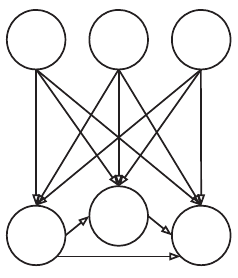
\includegraphics[height=3cm]{img/3_ML/mixed_model_FCL.png} \label{img:ML_mm_flc}}
    \subfigure[]{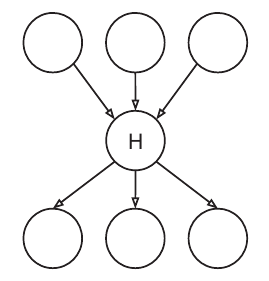
\includegraphics[height=3cm]{img/3_ML/mixed_model_LVM.png} \label{img:ML_mm_lvm}}
    \caption{Connections topology between the fully connected bayes network, where all conditional probabilities are explicitly assigned between each pair of the layers nodes with a total  (a), and the same model with a latent \textit{hidden} variable inserted between layers to represent conditional probabilities (b). }
    \label{fig:mixture_models}
\end{figure}
%
However once the \acs{LVM} is built the total number of parameters is significantly reduced in respect with the same model that directly represent correlation in the visible space. 



\subsubsection{linear factor analysis}
\label{linear factor analysis}
One problem with mixture models is that they only use a single latent variable to generate the
observations. In particular, each observation can only come from one of K prototypes. One can
think of a mixture model as using K hidden binary variables, representing a one-hot encoding
of the cluster identity. But because these variables are mutually exclusive, the model is still
limited in its representational power.
An alternative is to use a vector of real-valued latent variables, $z_i \in R_L$ . The simplest prior
to use is a Gaussian (we will consider other choices later):

% p(zi ) = N (zi |μ0 , Σ0 )

If the observations are also continuous, so $x_i \in R_D$ , we may use a Gaussian for the likelihood.
Just as in linear regression, we will assume the mean is a linear function of the (hidden) inputs,
thus yielding


% RR  VAE
Training this type of model has been a long-standing problem in the machine learning community, and classically, most approaches have had one of three serious drawbacks. First, they might require strong assumptions about the structure in the data. Second, they might make severe approximations, leading to sub optimal models. Or third, they might rely on computationally expensive inference procedures like Markov Chain Monte Carlo. More recently, some works have made tremendous progress in training neural networks as powerful function approximators through backpropagation \cite{NIPS2012_4824}. These advances have given rise to promising frameworks which can use backpropagation-based function approximators to build generative models. One of the most popular such frameworks is the Variational Autoencoder \cite{}, the subject of this tutorial. The assumptions of this model are weak, and training is fast via backpropagation. VAEs do make an approximation, but the error introduced by this approximation is arguably small given high-capacity models. These characteristics have contributed to a quick rise in their popularity

% RR
An autoencoder is a neural network that is trained to attempt to copy its input to its output. Internally, it has a hidden layer $h$ that describes a code used to represent the input. The network may be viewed as consisting of two parts: an encoder function $h=f(x)$ and a decoder that produces a reconstruction $r=g(h)$. If an autoencoder succeeds in simply learning to set $g(f(x))=x$ everywhere, then it is not especially useful. Instead, autoencoders are designed to be unable to learn to copy perfectly. Usually they are restricted in ways that allow them to copy only approximately, and to copy only input that resembles the training data. Because the model is forced to prioritize which aspects of the input should be copied, it often learns useful properties of the data.
%  _____ ___ _     _       _   _ _____ ____  _____ 
% |  ___|_ _| |   | |     | | | | ____|  _ \| ____|
% | |_   | || |   | |     | |_| |  _| | |_) |  _|  
% |  _|  | || |___| |___  |  _  | |___|  _ <| |___ 
% |_|   |___|_____|_____| |_| |_|_____|_| \_\_____|
%

%% ALL DIMENSIONALITY REDUCTION

% RR
Modern autoencoders have generalized the idea of an encoder and a decoder beyond deterministic functions to stochastic mappings $p_{encoder}(h | x)$ and $p_{decoder}(x | h)$.

%% TODO: TALK ABOUT GAN TOO

\subsection{Variational autoencoders and ELBO minimization}
\label{section:VAE}
% RR
In just three years, Variational Autoencoders (VAEs) have emerged as one of the most popular approaches to unsupervised learning of complicated distributions. VAEs are appealing because they are built on top of standard function approximators (neural networks), and can be trained with stochastic gradient descent.

% RR
Copying the input to the output may sound useless, but we are typically not interested in the output of the decoder. Instead, we hope that training the autoencoder to perform the input copying task will result in h taking on useful properties. One way to obtain useful features from the autoencoder is to constrain h to have a smaller dimension than x. An autoencoder whose code dimension is less than the input dimension is called \textbf{undercomplete}. Learning an undercomplete representation forces the autoencoder to capture the most salient features of the training data.


In \cref{section:feedforward dense networks} we showed that a neural network can be also seen in a Bayesian description as a problem of conditional probability, where we are interested in the posterior description of a dataset. A very commonly exploited method to infer that posterior distribution is \textit{Variational Inference}~\cite{Jordan:1999:IVM:339248.339252}~\cite{MAL-001}. It has been proposed an alternative strategy to \ac{MCMC} sampling because tends to be faster to train and easier to scale with large datasets.

If we start by considering a joint density of latent variables $\bm{z} = [z_1, z_2, ...,z_m]$ and observations $\bm{x} = [x_1, x_2, ..., x_n]$:
\begin{equation}
    p(\bm{z},\bm{x}) = p(\bm{z}) p(\bm{x}|\bm{z})
\end{equation}
Applying the Bayes rule we can relate latent variables, with their prior $p(\bm{z})$ distribution, to the observations through:
\begin{equation}
    p(\bm{z}|\bm{x}) = \frac{p(\bm{z})p(\bm{x}|\bm{z})}{p(\bm{x})}
\end{equation}
where $p(\bm{x}|\bm{z})$ is defined as the data \textbf{likelihood}, $p(\bm{z}|\bm{x})$ the \textbf{posterior} distribution, while
\begin{equation}
    p(\bm{x}) = \int_{\mathbb{R}^Z} p(\bm{z}, \bm{x}) d\bm{z}
\end{equation}
is usually referred as the \textbf{evidence} and it can be obtained by marginalization of the latent space from the joint density.

While in \acl{MCMC}, we build an ergodic Markov Chain on $\bm{z}$ for which the stationary distribution is the posterior; then we collect a number of samples from the posterior through the chain, and we approximate the posterior with an empirical estimate from the samples (the more dense are the samples, the higher the probability in that region).
Rather than sampling, the main idea behind \textit{Variational Inference} is to use optimization: given a possible set of functions of approximate densities $\mathcal{Q}$, we try to find the members of this set (i.e. the proper set of parameters once the family is defined by a parametrical functional) that minimizes the distance to the exact posterior. So from this new density $q(\bm{z})$, e can be measure the distance as the Kullback-Leibler divergence with $p(\bm{z}|]\bm{x})$; and the optimization looks for:
\begin{equation}
    \tilde{q}(\bm{z}) = \argmin{q(\bm{z}) \in \mathcal{Q}} \KLD{q(\bm{z})}{p(\bm{z}|\bm{x})}
    \label{eq:variational_inference}
\end{equation}
where the KL divergence is defined as:
\begin{equation}
    \KLD{q(\bm{z})}{p(\bm{z}|\bm{x})} = \expectation{\log q(\bm{z})}_{q(\bm{z})} - \expectation{\log p(\bm{z}|\bm{x})}_{q(\bm{z})}
    \label{eq:kulback-leibler}
\end{equation}
The idea is, as stated, to turn a inference problem into an optimization process; while the family of chosen functions handle the quality of the minima in KL distance. One of the key points on this approach is indeed to pick a set of functions $\mathcal{Q}$ that is general enough to guarantee an efficient optimization but also flexible enough to capture the posterior details.

\subsubsection{The evidence lower bound}
We just saw that variational inference seek for a proper candidate to solve \eqref{eq:variational_inference}, so once found the $\tilde{q}(\bm{z})$ it sets that function as the \textit{best approximation} of the posterior. Unfortunately this is not describable in a closed form because the \textit{evidence} depends on the joint probability with inaccessible latent variables.
So we expand the conditional in \cref{eq:kulback-leibler} as:
\begin{equation}
    \KLD{q(\bm{z})}{p(\bm{z}|\bm{x})} = \expectation{\log q(\bm{z})}_{q(\bm{z})}
                                        - \expectation{\log p(\bm{z},\bm{x})}_{q(\bm{z})} 
                                        + \log p(\bm{x})
\end{equation}
where the last term came out of the expectation because it does not depend on $\bm{z}$. 
We define as the negative \ac{ELBO} the part of RHS of the equation that depends on $q(\bm{z})$, so:
\begin{equation}
    \KLD{q(\bm{z})}{p(\bm{z}|\bm{x})} = - \mathrm{ELBO}_{q(.)} + \log p(\bm{x})
\end{equation}
so \acs{ELBO} is:
\begin{align*}
    \mathrm{ELBO}_{q(.)} &= \expectation{\log p(\bm{z},\bm{x})}_{q(\bm{z})} - \expectation{\log q(\bm{z})}_{q(\bm{z})} \\
                         &= \log p(\bm{x}) - \KLD{q(\bm{z})}{p(\bm{z}|\bm{x})} 
\end{align*}
And being the KL term a distance is also positive definite so:
\begin{equation}
    \log p(\bm{x}) \geqslant \mathrm{ELBO}_{q(.)}
\end{equation}
so it defines a lower bound of the distance residual we can get in matching the posterior, hence the name. So what we obtained is that to have an approximation function such that the KL distance is minimal, with respect to the choice of the particular function $q(.) \in \mathcal{Q}$, we need "at least" to maximize the \acs{ELBO} addendum.
To do this we expand its first term using the definition of conditional probability:
\begin{align*}
    \mathrm{ELBO}_{q(.)} &= \expectation{\log p(\bm{z},\bm{x})}_{q(\bm{z})} - \expectation{\log q(\bm{z})}_{q(\bm{z})} \\
                         &= \expectation{\log p(\bm{x}|\bm{z})}_{q(\bm{z})} + \expectation{\log p(\bm{z})}_{q(\bm{z})} - \expectation{\log q(\bm{z})}_{q(\bm{z})} \\
                         &= \expectation{\log p(\bm{x}|\bm{z})}_{q(\bm{z})} + \KLD{q(\bm{z})}{p(\bm{z})}
\end{align*}
We can now make a little digression on this result: the first term of the last equation is a likelihood expectation so it encourages densities that place their mass on latent variables that explain the observed data. The second term is the negative value of KL divergence between the variational density and the prior; so it encourages densities that are close to the prior. 
Thus optimizing \acs{ELBO} means making the Bayes balance between likelihood and prior for the training dataset.
%
\begin{figure}
    \centering
    \subfigure{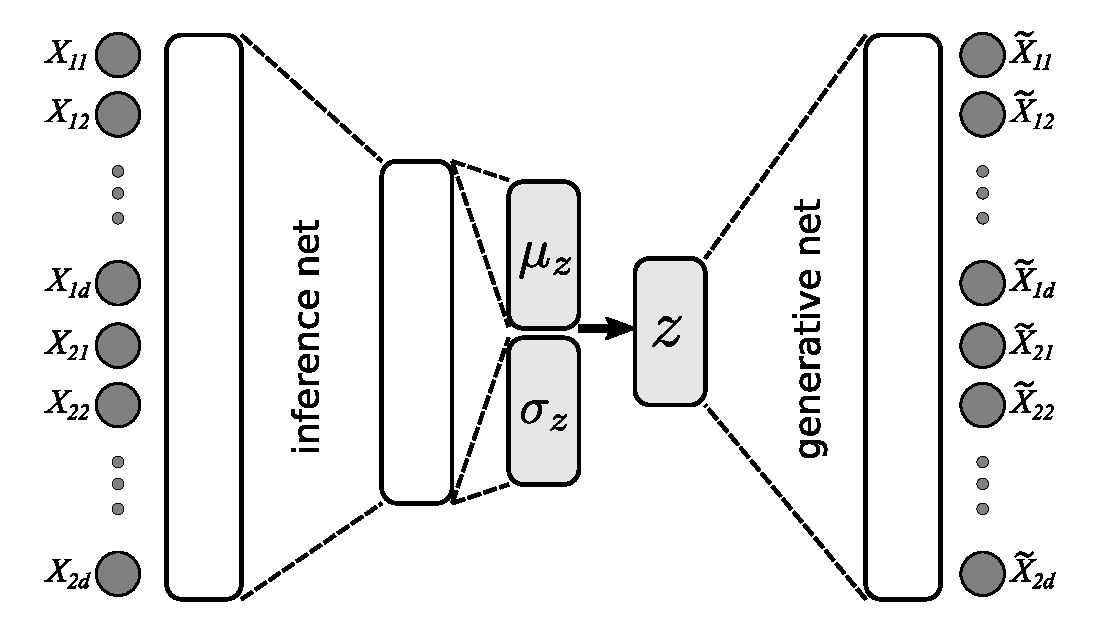
\includegraphics[height=4.5cm]{img/3_ML/VAE_1.pdf} \label{fig:step1_vae}}
    \subfigure{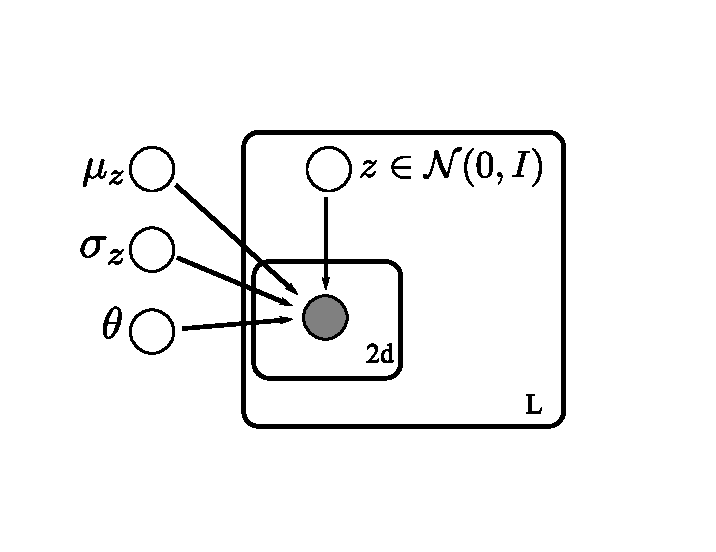
\includegraphics[height=4.5cm]{img/3_ML/VAE_1_plate.pdf} \label{fig:step1_vae_plate}}
    \caption{ The general description of a Variational Autoencoder shown both in its topological structure (left sketch), where the encoder and decoder are connected by inner reparametrization layers that form the inner latent space variables; and in \textit{plate notation} where all covariates are explained through latent variables (hidden "causes") with normal distribution. }
    \label{fig:step_1_VAE}
\end{figure}










%  _____ ___ _     _       _   _ _____ ____  _____ 
% |  ___|_ _| |   | |     | | | | ____|  _ \| ____|
% | |_   | || |   | |     | |_| |  _| | |_) |  _|  
% |  _|  | || |___| |___  |  _  | |___|  _ <| |___ 
% |_|   |___|_____|_____| |_| |_|_____|_| \_\_____|
%


\section{Latent space topology}

To provide a good playground for the tests that we initially foresaw for this study we built a simple algorithm to simulate possible dataset of one-dimensional signals. This may seem quite naive with respect to complex \acs{DNN} inputs that characterize the latest works presented in this field, however this turns to worth for our purposes. Indeed it is very simple to manage and matches the simple case of the feature extraction applied to the acquisition device that we plan to add to experiment \acs{DAQ} system. Moreover it present a quite widespread application in the area of signal conditioning allover the experiment diagnostics: both in the temporal domain and in the spatial domain. For example the \acs{SXR} - that is our main case of study - provides at outputs a one-dimensional signal representing the spatial distribution of the electronic temperatures $T_e$ at time $t$. All measures in this case are computed by measures of the integrated signal along the cords, and inverted to find the actual point temperature that is finally projected on the central axis in the equatorial plane crossing the the center of the machine and the center of the chamber. The final output is a set of ordered points that can vary in: number (missing points for non working chords), position along projection axis, and temperature value.

\subsection{Gaussian sum generator}
\label{section: gaussian sum generator}
As a first very general approach we just created an automatic generator of a one-dimensional sum of Gaussians envelopes. 
The generator is lead from a set of parameters, such as: the number of points to generate, the random distribution of possibly missing values, the fixed missing positions, the added generation noise, and so forth. 
Once the generator is queried for a new instance it selects randomly a label number that corresponds to a particular curve in a defined set of function classes. For the definition of gaussians we use a dictionary named \textit{kinds} that provides, for each possible label, a set of arrays in \textit{gain},  \textit{mean}, and \textit{sigma} for each of the sum of Gaussians components.
In \Figure{\ref{fig:sum_of_gaussians}} an example of five \textit{kinds} setup (aka reconstruction labels) is shown with their respective representation curves. 
%
\begin{figure}
    \centering
    \begin{minipage}[b]{0.57\textwidth}
    \begin{lstlisting}[
        language=Python,
        basicstyle=\tiny,
        numbers=none,
    ]
 from Dummy_g1data import Dummy_g1data
 
 ds = Dummy_g1data( feature_dim=40, 
                    latent_dim=2, 
                    counts=10000 )
 ds.kinds = [
  {'gain': [1, 1],'mean': [0.2, 0.8], 'sigma': [0.1, 0.1]},
  {'gain': [0.5], 'mean': [0.8], 'sigma': [0.1]},
  {'gain': [0.5], 'mean': [0.2], 'sigma': [0.1]},
  {'gain': [1],   'mean': [0.5], 'sigma': [0.2]},
  {'gain': [0.5], 'mean': [0.5], 'sigma': [0.2]}
 ]
 ds.buffer() # buffer 10K samples in memory
 
 # adapt dataset generator to VAE with labels as input
 ds = ds.ds_array.map(lambda x,k: (x,x) )
 
 
    \end{lstlisting}
    \end{minipage}
    \hfill
    \begin{minipage}[b]{0.42\textwidth}
     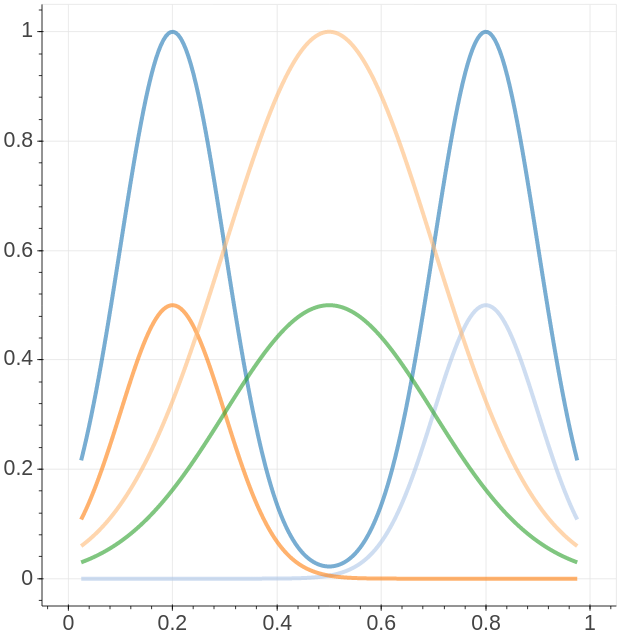
\includegraphics[height=5cm]{img/STEP1/dummy_kinds.png}
    \end{minipage}
    \caption{A generation setup example for five \textit{kinds} of sum of gaussians: on the left the dictionary taht fills the parameters of the generator for each of the five classes; on the right a plot shows the five kind representations where colours helps to distinguish among them. }
    \label{fig:sum_of_gaussians}
\end{figure}
%
The generation of each dataset instance proceeds as described in the following. At first we chose an ordered set of values along x-axis from a uniform distribution $\bm{x}_1 \in \mathbb{R}^{d}$ (with $x_{1,i} \geq x_{1,i-1}$), where $d$ is the number of desired points generated for each instance. Then, if not specifically asked, a label is also extracted form uniform random integers within the range of \textit{kinds} cardinality; and the related Gaussian exponential is applied for each of the parameter in that \textit{kind} and for each of the points. So a new set $\bm{x}_2 \in \mathbb{R}^d$ is created, in which:
\begin{equation}
    \bm{x}_2 = \sum_{k=1}^K \frac{1}{Z_k} \exp{-\frac{1}{2}\left( \frac{\bm{x}_1-\mu_k}{\sigma_k}\right)^2}
\end{equation}
The complete data sample we use as input will now be \textbf{any} combination of $\{\bm{x}_1, \bm{x}_2\}$; for simplicity we chose to construct data with the simple concatenation: $\bm{x} = [\bm{x}_1, \bm{x}_2]$ where now $\bm{x} \in \mathbb{R}^{2d}$.
The generator is configured as a tensorflow dataset that is is directly fed into the autoencoder where we previously mapped \textit{data} and \textit{label} of each element both with $x$ vlaues (we are not interested in label as VAE is an unsupervised method) to train \acs{VAE} with proper matching input and output.
A possible minimal configuration of data generator is shown in \Figure{\ref{fig:sum_of_gaussians}} where we have five classes of curves in the range $x_i \cap [0,1]$. The same set of curves are also plotted in dense domain to provide a ground-truth for plots. We chose to train a \acs{VAE} with only \textbf{two latent variables} (hereafter indicated as \VAE{2}), this was only motivated by the fact that the result is easier to represent by Cartesian axes. This actually limits the latent space representational power, but this will be discussed in a proper section.
%
\begin{figure}
    \centering
    \subfigure{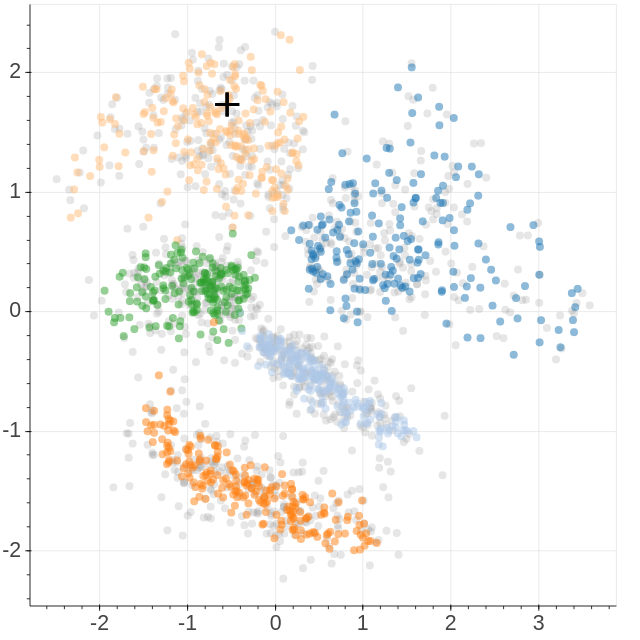
\includegraphics[height=4.5cm]{img/STEP1/ls1.png} \label{step1_1}}
    \subfigure{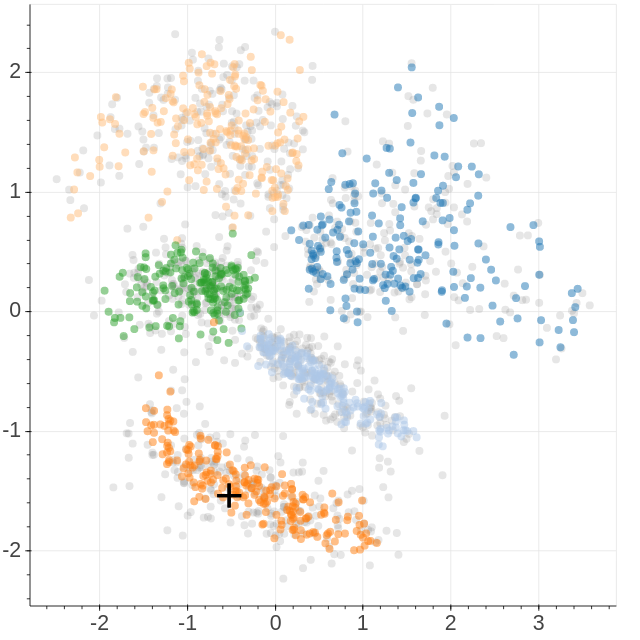
\includegraphics[height=4.5cm]{img/STEP1/ls2.png} \label{step1_2}}
    \subfigure{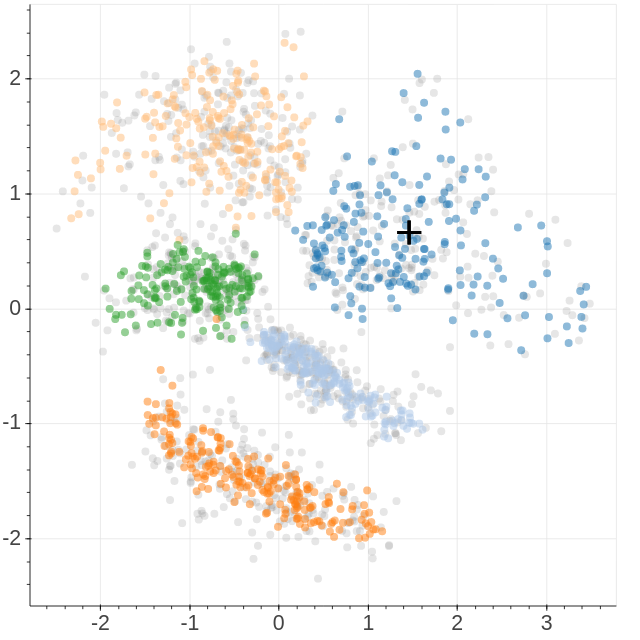
\includegraphics[height=4.5cm]{img/STEP1/ls3.png} \label{step1_3}}
    \subfigure{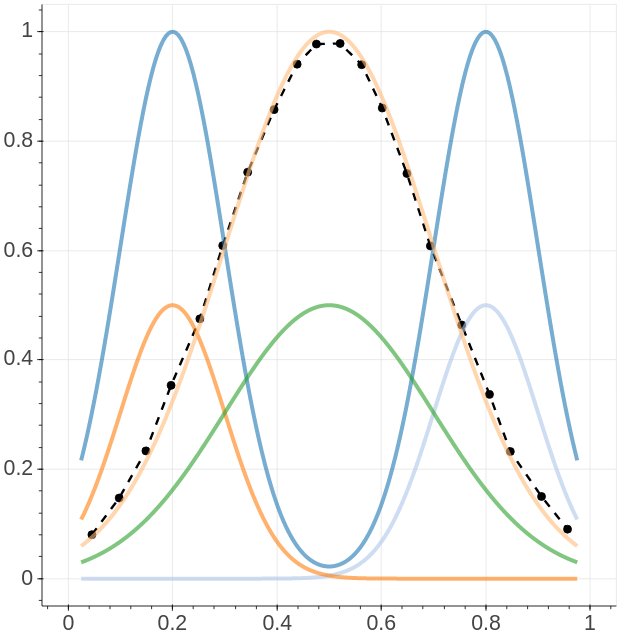
\includegraphics[height=4.5cm]{img/STEP1/gn1.png} \label{step1_4}}
    \subfigure{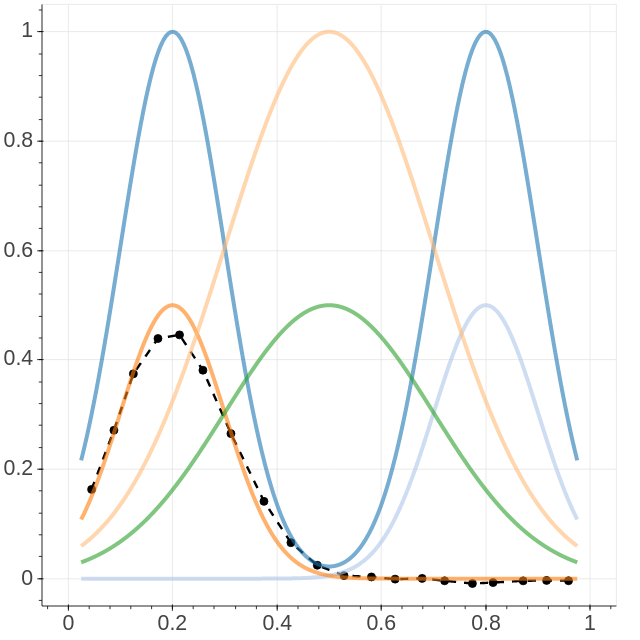
\includegraphics[height=4.5cm]{img/STEP1/gn2.png} \label{step1_5}}
    \subfigure{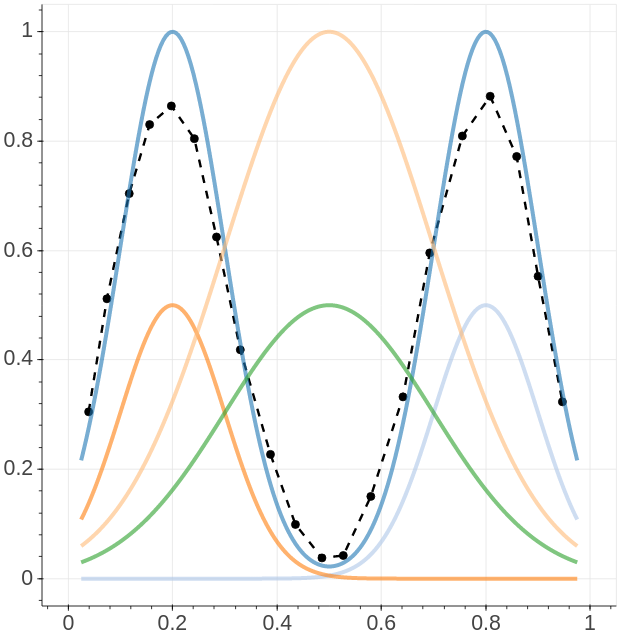
\includegraphics[height=4.5cm]{img/STEP1/gn3.png} \label{step1_6}}
    \caption{ Three instances of latent space reconstruction from \VAE{2} starting from a latent position indicated with ($\bm{+}$) in the scatter plot on top that corresponds to the black curve from decoder output plotted on bottom. In the upper figures the scatter plot shows also 1000 samples from validation dataset where the colour position shows the encoded mean $\bm{\mu}_z$ and the corresponding class in the colour scale), while the grey plot is a reconstruction of the $\bm{\sigma}_z$. The clusters color is also matching the corresponding \textit{kind} of curve that is plotted for reference on bottom figures.} 
    \label{fig:step_1}
\end{figure}
%
In \Figure{\ref{fig:step_1}} three examples of \acs{VAE} reconstruction have been plotted. The parameters for the generator were $d=20$, no generation noise have been applied and the latent space is 2-dimensional. Latent space variables $\bm{z}$ are characterized by their variational parameters, i.e. $\bm{\mu}_z$ and $\bm{\sigma}_z$, and those parameters are plotted in the same figure for the three examples in the top set of graphs for 1K samples of the validation dataset. The scatter plot shows a coloured dot corresponding  the inferred latent position in \textit{xy-axis} and the corresponding \textit{kind} on the colour scale. A further grey dot is also plotted for each of the latent samples after the variational has been applied to generate a Monte Carlo approximation of the training process $\mathcal{N}(\bm{\mu}_z, \bm{\sigma^2}_z)$.
The same figure shows also a instance of the generative network output with black dots in the lower plots that have been overimposed to the ground-truth curves \textit{kinds} to see the matching. The reconstruction corresponds to the black cross ($\bm{+}$) in the latent space. It is worth to highlight the fact that this ($\bm{+}$) point was a generated point in the latent space and does not corresponds to any sample of either the training set or the validation set. it is a new \textit{unseen} generation instance that lies within the latent space in the corresponding class cluster, but from the trained generator point of view, there is actually any more correlations with the input data; this also corresponds to the Bayes idea where the generated instance are only related with the latent "cause", once we fixed the trained parameters (see plate notation in \Figure{\ref{fig:step1_vae_plate}}).
Those plot have been generated using the utility functions we implemented for \RFXhunch exploiting the \textit{Bokeh}~\cite{bokeh} library for python and JavaScript; this can provide a useful scope to see the behavior of the decoder moving interactively the point in the 2D latent space ans looking at the reconstruction on the generated plot.
The complete \RFXhunch package will be described with more detail in \cref{section:RFXhunch}.
%
\subsection{generative morphing effect}
When we play with joint encoder/decoder networks, that are our tools to step in and out of the latent space, \acs{VAE} is thought as a directed \acs{RBM}, and it is claimed to extract a meaning from data by extracting latent "concepts" and expanding them to the feature space. On the other hand we already pointed out that the generative effect of \acs{VAE} is also that, once trained, it maintains any actual relation with the data and can generate samples by only means of decoding the latent space. This becomes clear if we sample a point that is far from the dataset encoded clusters; for example in \Figure{\ref{fig:step1_morph}} two latent space points ($\bm{z}_1$ and $\bm{z}_2$) have been reconstructed by generative network. 
%
\begin{figure}
    \centering
    \subfigure{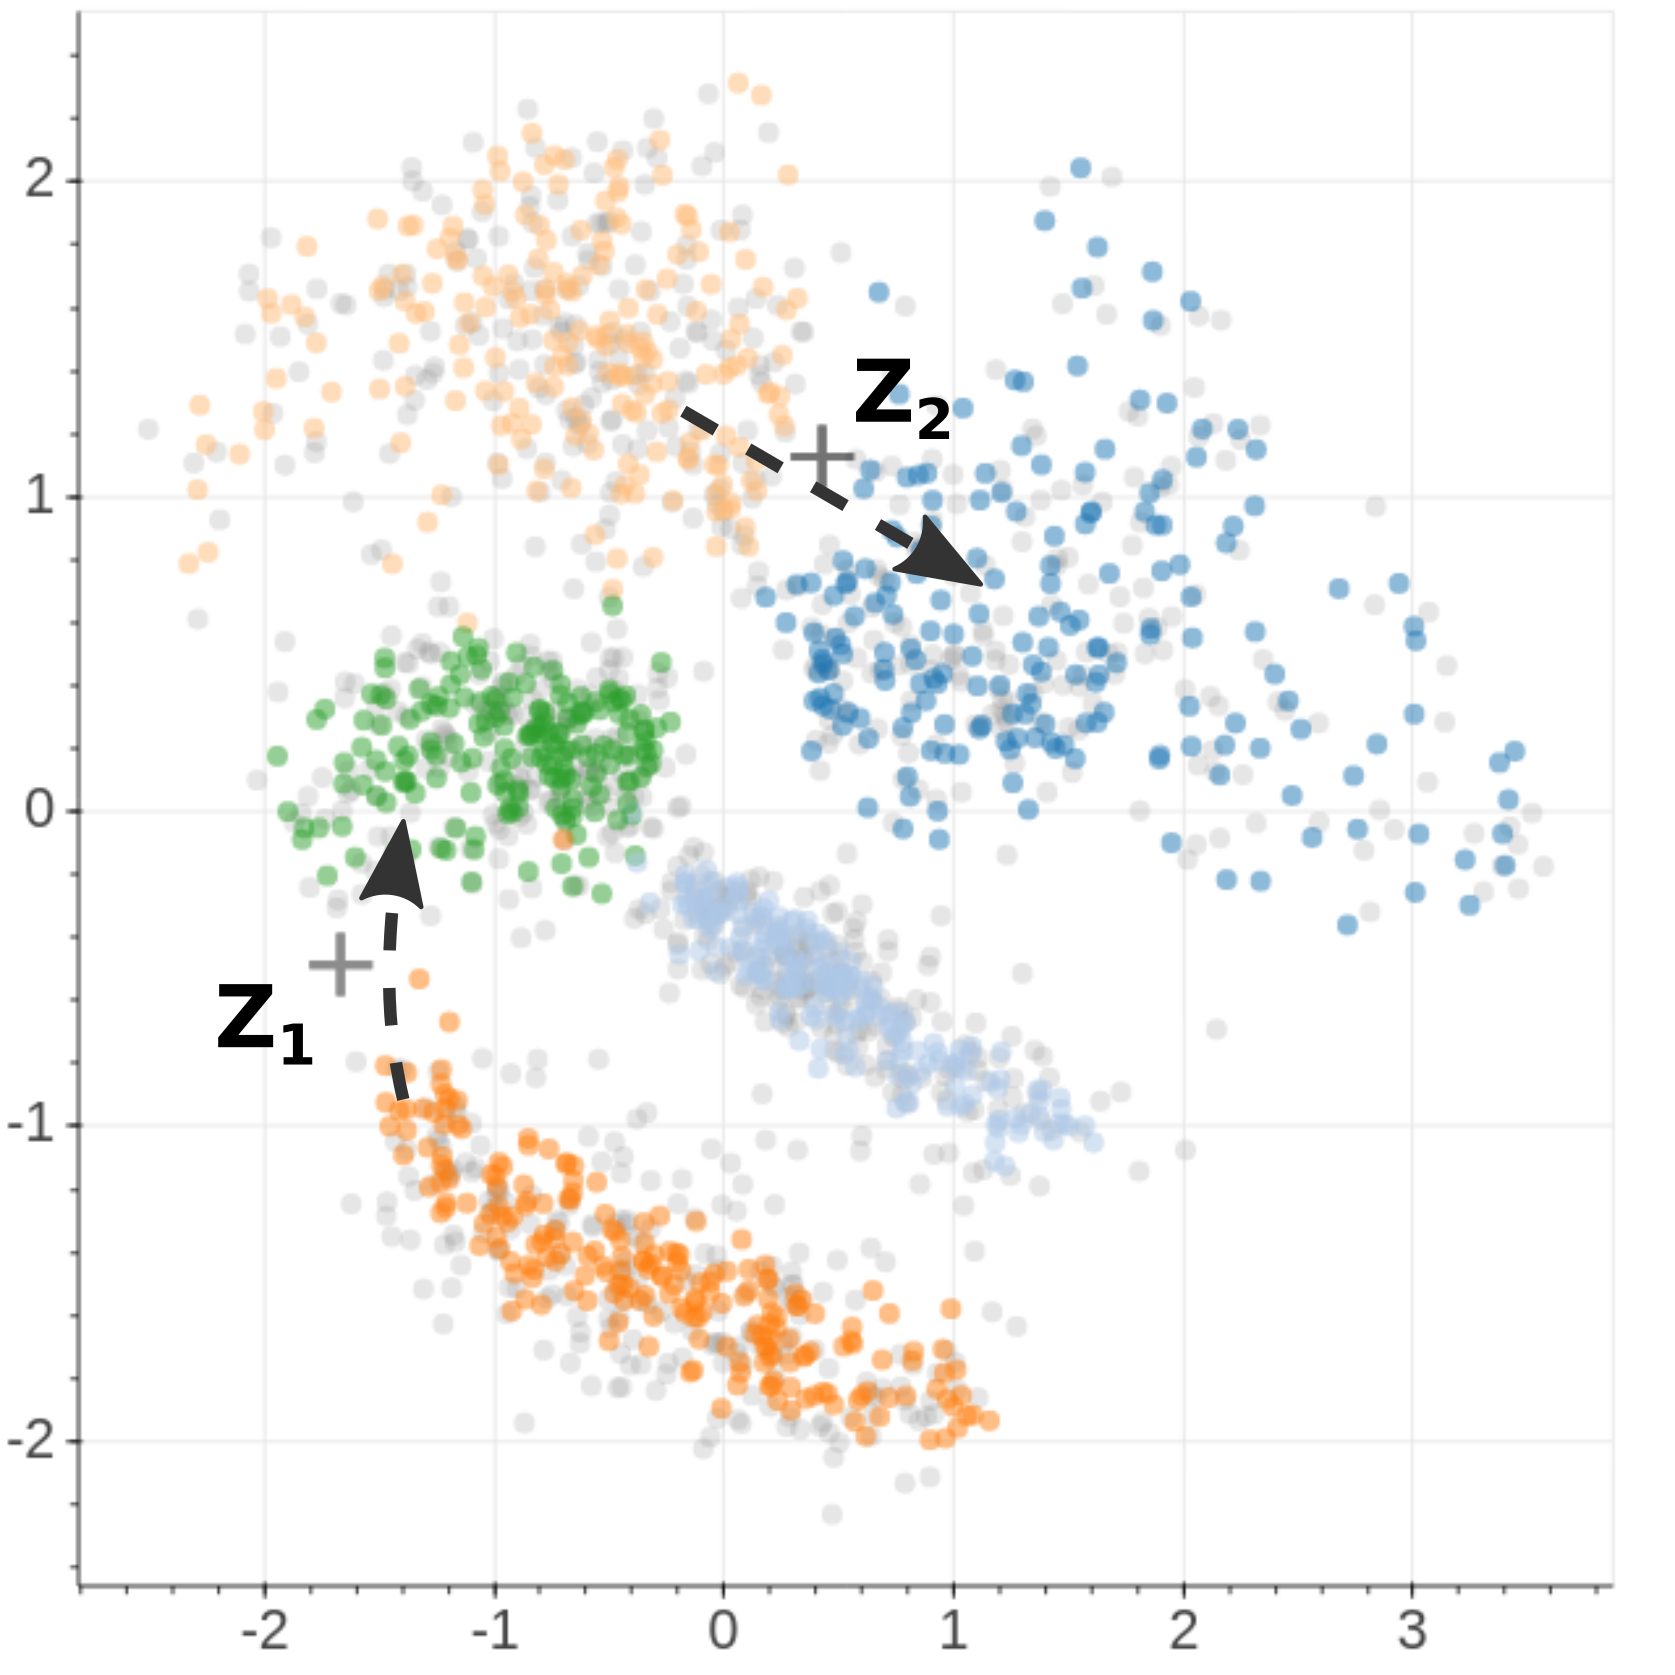
\includegraphics[height=4.5cm]{img/STEP1/morph_Z1Z2.png}\label{fig:step1_morph_z1z2}}
    \subfigure{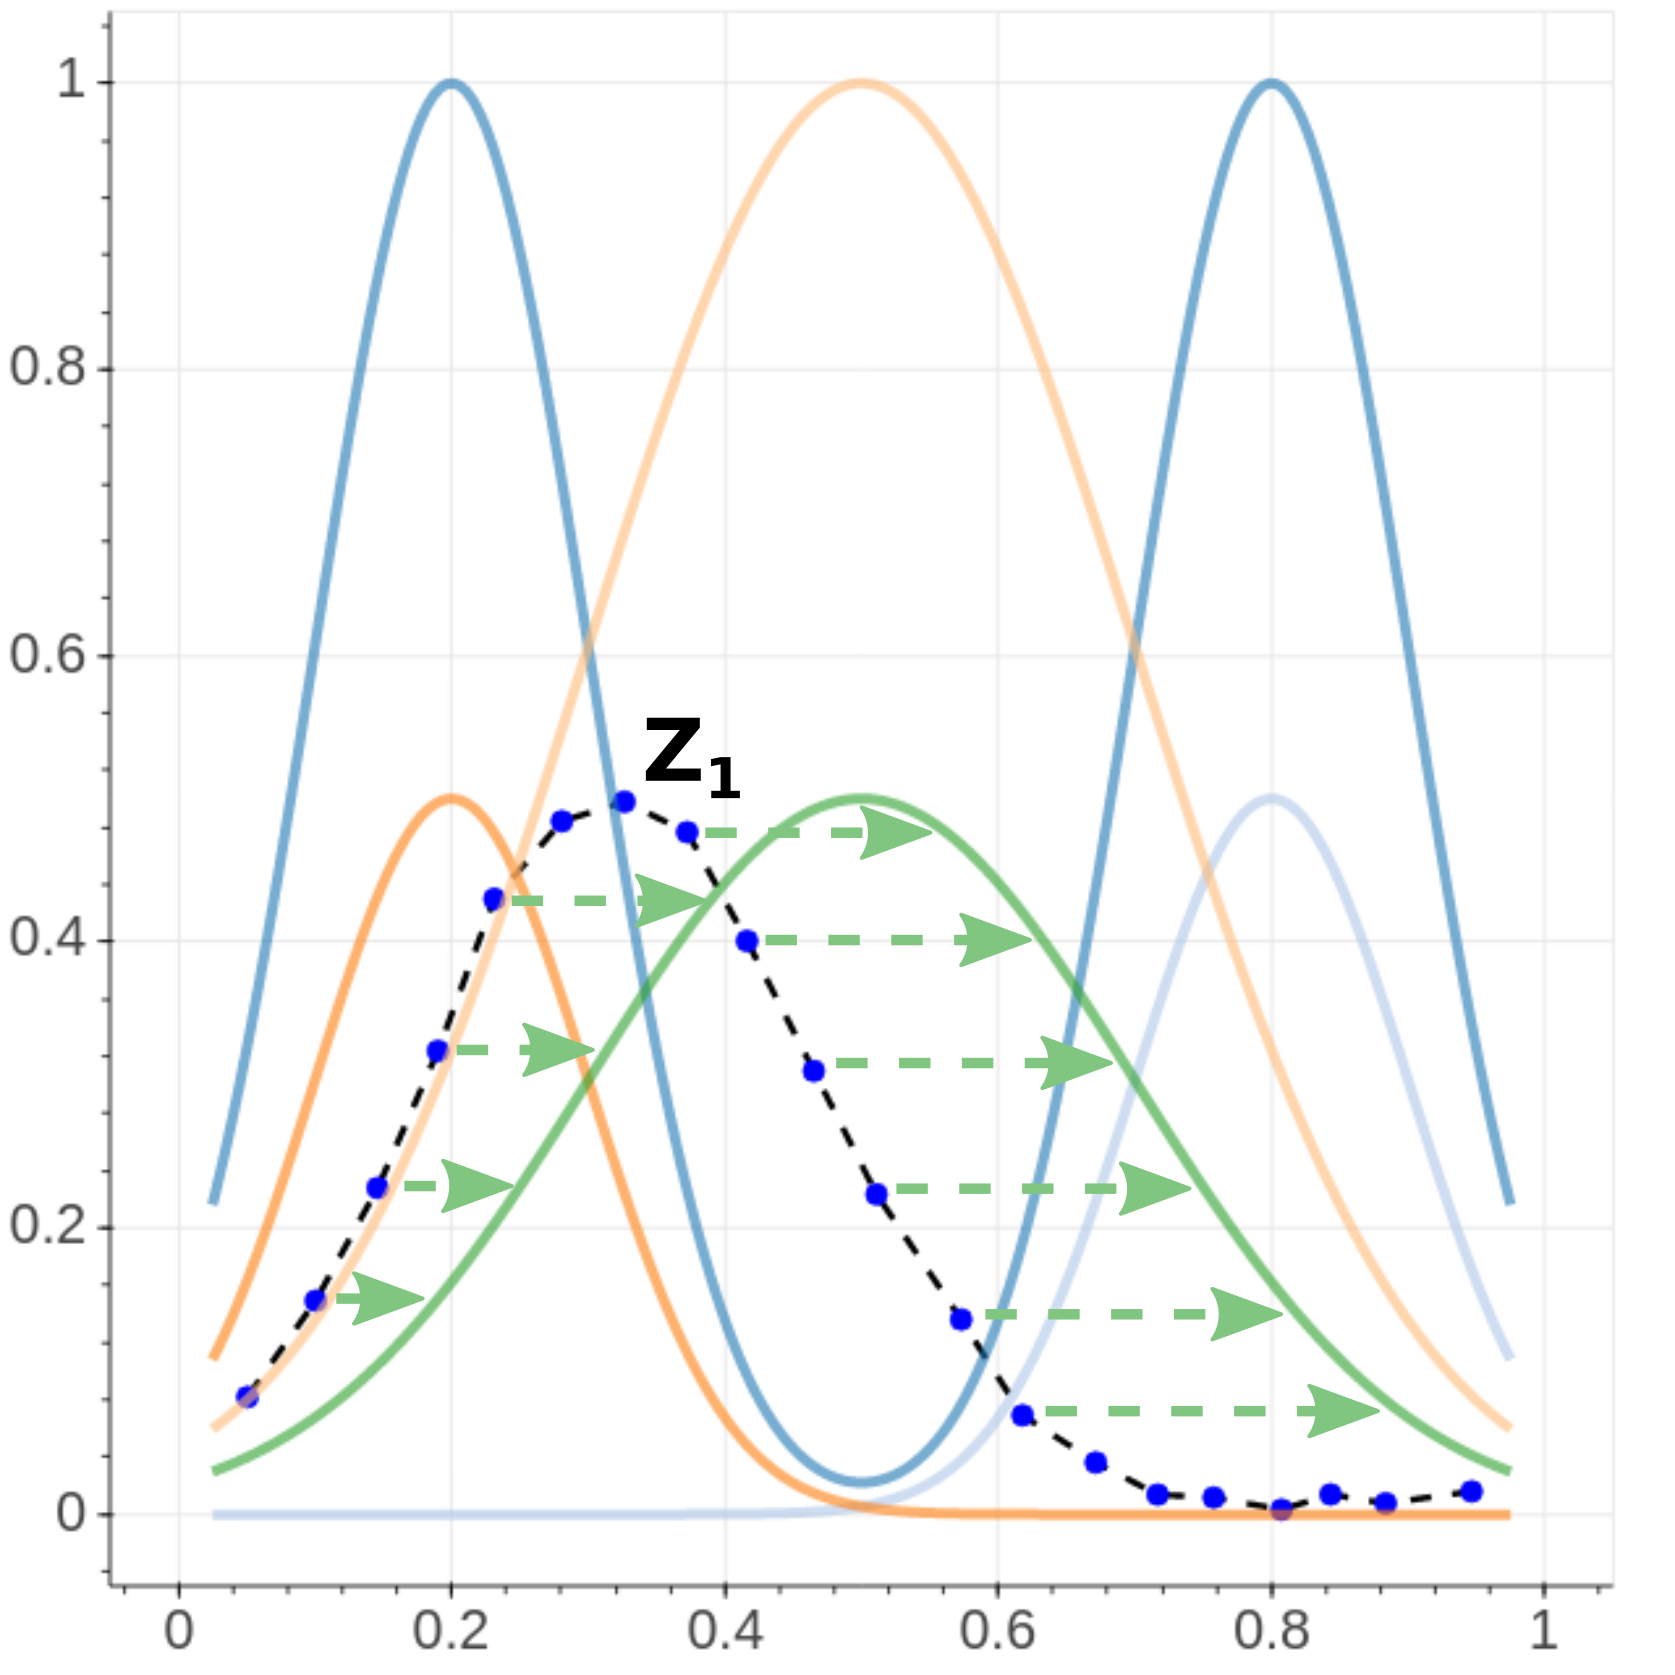
\includegraphics[height=4.5cm]{img/STEP1/morph_gn2.png} \label{fig:step1_morph_gn2}}
    \subfigure{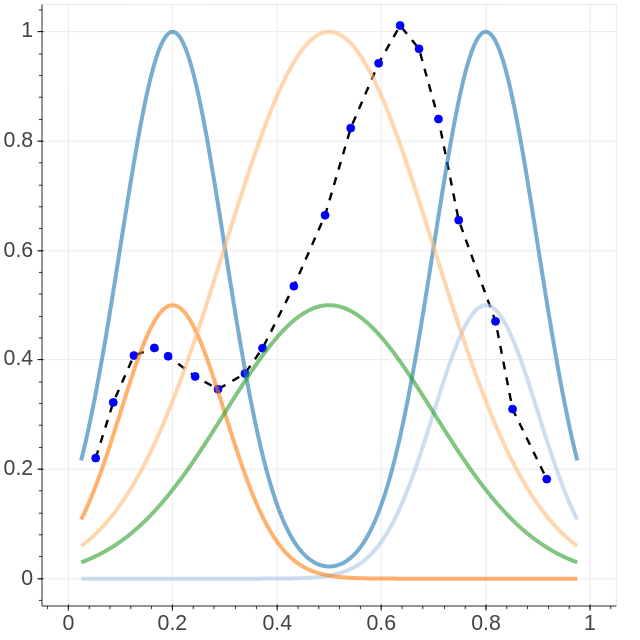
\includegraphics[height=4.5cm]{img/STEP1/morph_gn4.png} \label{fig:step1_morph_gn4}}
    \caption{Generative morph effect on reconstruction from \VAE{2}: two latent space point taken from middle space between clusters has been decoded and show how the generative effect can create solution for non existent data "morphing" one class to another. } 
    \label{fig:step1_morph}
\end{figure}
It is quite clear from these figures the real power of the latent space, if we paint the reconstructed signal from any point in the latent space we just traversed all possible configuration that the outputs will assume, so once we know how this space is shaped we can lead the output to maintain certain characteristics. For instance we can constrain the system to remain within some predefined boundaries thus implementing a very simple, but robust, non linear control on the outputs.

\subsection{latent space topology}
With the description of \textit{linear factor analysis} in \cref{linear factor analysis} the unidentifiability of the latent variables has been introduced; so unfortunately upon each training the latent space assumes a different configuration. 
Nonetheless, beside the simple generation on points that lies in the latent "\textit{interstitial}", one start to think about which possible configurations the latent space itself could assume. Given the fact that the purpose of \acs{VAE} is to adapt the space upon jumps between clusters of similar features, the idea is that we could imagine to simplify the entire cluster with its center of mass, and separate the space itself in corresponding regions. This could be easily done with the unsupervised k-means algorithms with k corresponding to the k classes ( the \textit{kinds} ) and let it find the means for each center of mass. At this point we could have an algorithm that actively classify the features upon latent representation, while in the latent space this classification can be plotted by the classical \textit{Voronoi diagram} as shown in \Figure{\ref{fig:voronoi_ls}}. With this defined regions we can say that a curve is of a certain class if its latent coordinates are within the corresponding region $k_i$; but what happens in the boundaries? In the previous section it has been shown that the algorithm tends to make a morphing adjustment to the signal shape to make the step from one region to the other as smooth as possible, however it is not always a feasible solution. For instance, as it can be seen in \Figure{\ref{fig:step1_morph_gn4}}, passing from the central Gaussian curve to the double one requires a steep movement on the position of generated points.
Although the topological configuration of the latent space remain generally unidentifiable, and so does the clusters organization, deep looking back at \Figure{\ref{fig:step_1}} an overall structure among the samples placed by the encoder in the scatter plot can be glimpsed. For example the two single Gaussian curves that have been defined at plot center (i.e. the curve generated from the last two \textit{kinds}: $k_4, k_5$), corresponding respectively to the $\bm{A}$ cluster (green) and the $\bm{B}$ cluster (top light-orange) have been placed close to each other. And this configuration repeats with high probability with different trainings; this happens because the algorithm finds "easy" to generate a transition from the these two classes, that is the total amount of point movements remained small for each of the training attempt. The same happens for the tree curves at the lower part of the plot: the left orange (\textbf{E}), the previous central green one (\textbf{A}), and the azure one (\textbf{D}). In addition, the shift transition of the Gaussian points protrusion from left to right is actually a "C" shape curve in latent space because the algorithm chose to guarantee the transition from $\bm{D}$ to $\bm{E}$ as well. That because the total cost (meant as the integral of the computed loss) associated with that transition ( i.e. the rise of the bent on one side and the fall of the bent in the other) is also small with respect to other transitions. On the contrary a complete symmetry should exist between the transition from curve \textbf{D} to \textbf{C} and from curve \textbf{E} to \textbf{C}, so those groups of samples could be thought to be equally close to each other; but the training decided for one or the other arrangement because it is associated to a steeper change on reconstructed points than the other solutions. A natural parallelism of such cost transition with the field theory could be argued and indeed a perturbation approach to the study of latent space structure has been recently proposed in~\cite{andrsterr2019perturbation}. Associating an energy jump upon classes helps to identify which are the main degrees of freedoms for the latent variables in performing transitions or any movement in the latent space( remember that we are not bounded to the simple case of multi-class classification).
In \Figure{\ref{fig:voronoi_2d}} a connected graph has been drawn to plot all possible transitions among classes of the reported example, that is actually the dual representation of the Voronoi diagram of \Figure{\ref{fig:voronoi_ls}}. Imaging each edge as the minimum energy path to cross the boundary between two classes, the number of possible free edges would be strictly linked with the latent space dimensionality: for 1-dimensional latent space 3 classes can be represented, 4 classes can represented with a 2-dimensional space and 5 classes with a 3-dimensional space, and so forth. 
The idea behind this is the possibility to draw a graph with no crossing edges to create a smooth transition with any possible couple of knots in the graph. However because the actual crossing edges between clusters can be associated with the energy of the system configuration, there can be solutions where the same configuration can explain many edges; an example is provided by the proposed set of classes where transitions $\bm{A} \rightarrow \bm{C}$, and $\bm{B} \rightarrow \bm{D}$ are matching with a unique representation in a crossing point. 
Conversely, the only way for $\bm{E}$ to reach $\bm{C}$ would be to spreading around either $\bm{D}$ or $\bm{A}\cup\bm{B}$ with a sensible loss of energy for the cluster that would fade out the description of the $k_3$ covariates, thus being unfeasible for the optimum representation reached by the \acs{VAE}.
In any case the distance between $\bm{E}$ and the other clusters represents a limit on the overall optimization, and a possible way around this limitation is to increase the dimensionality of latent space (i.e. the number if the embedding neurons) as proposed in~\Figure{\ref{fig:voronoi_3d}}.
\begin{figure}
    \centering
    \subfigure{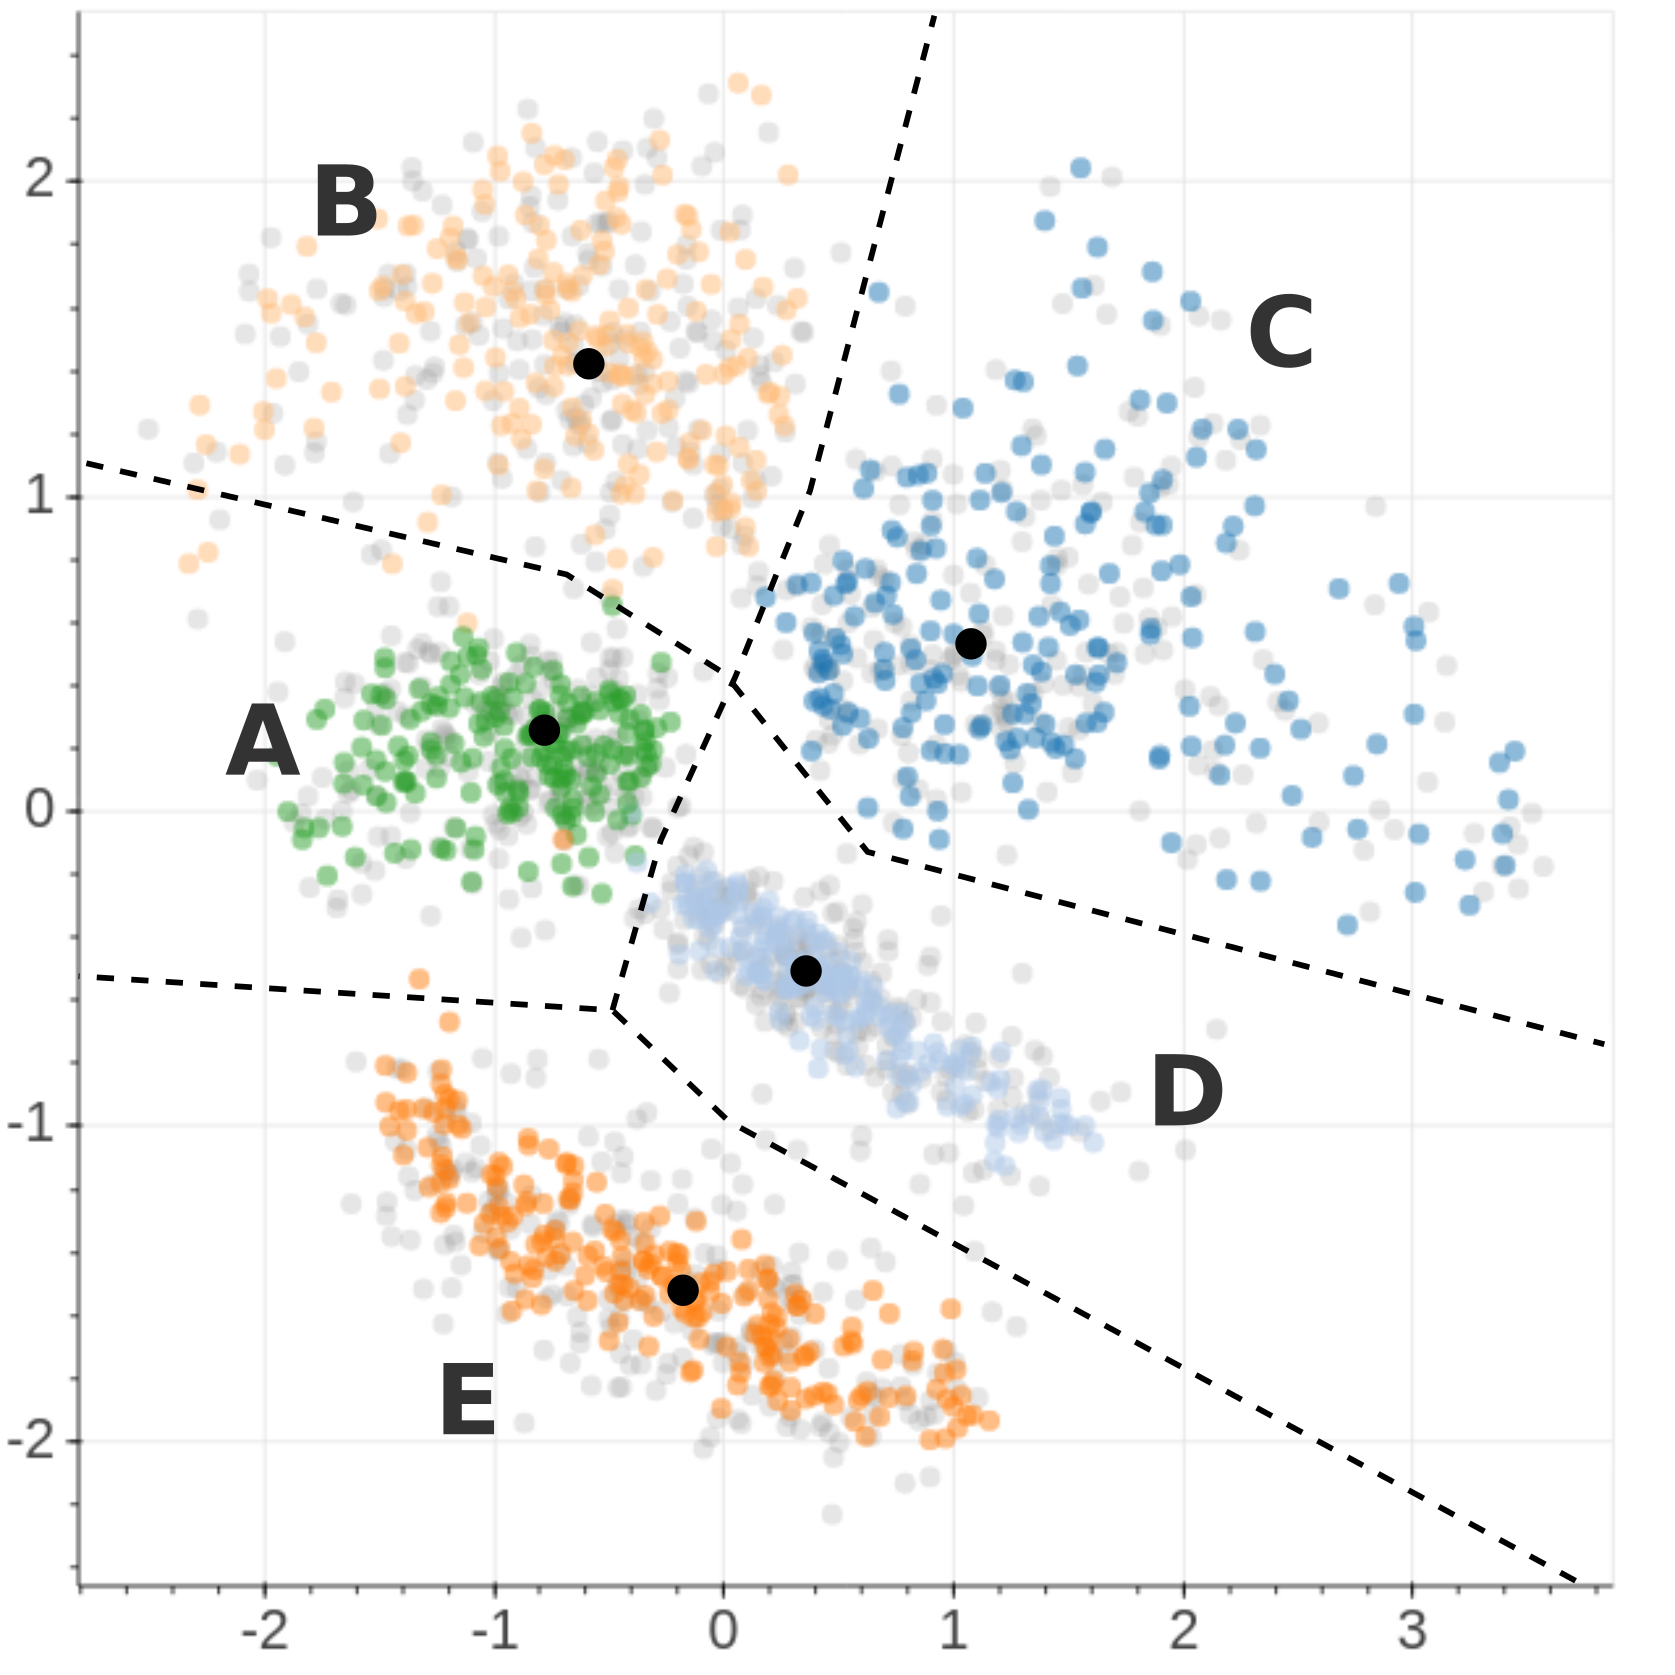
\includegraphics[height=4.5cm]{img/STEP1/voronoi_ls.png}\label{fig:voronoi_ls}}
    \subfigure{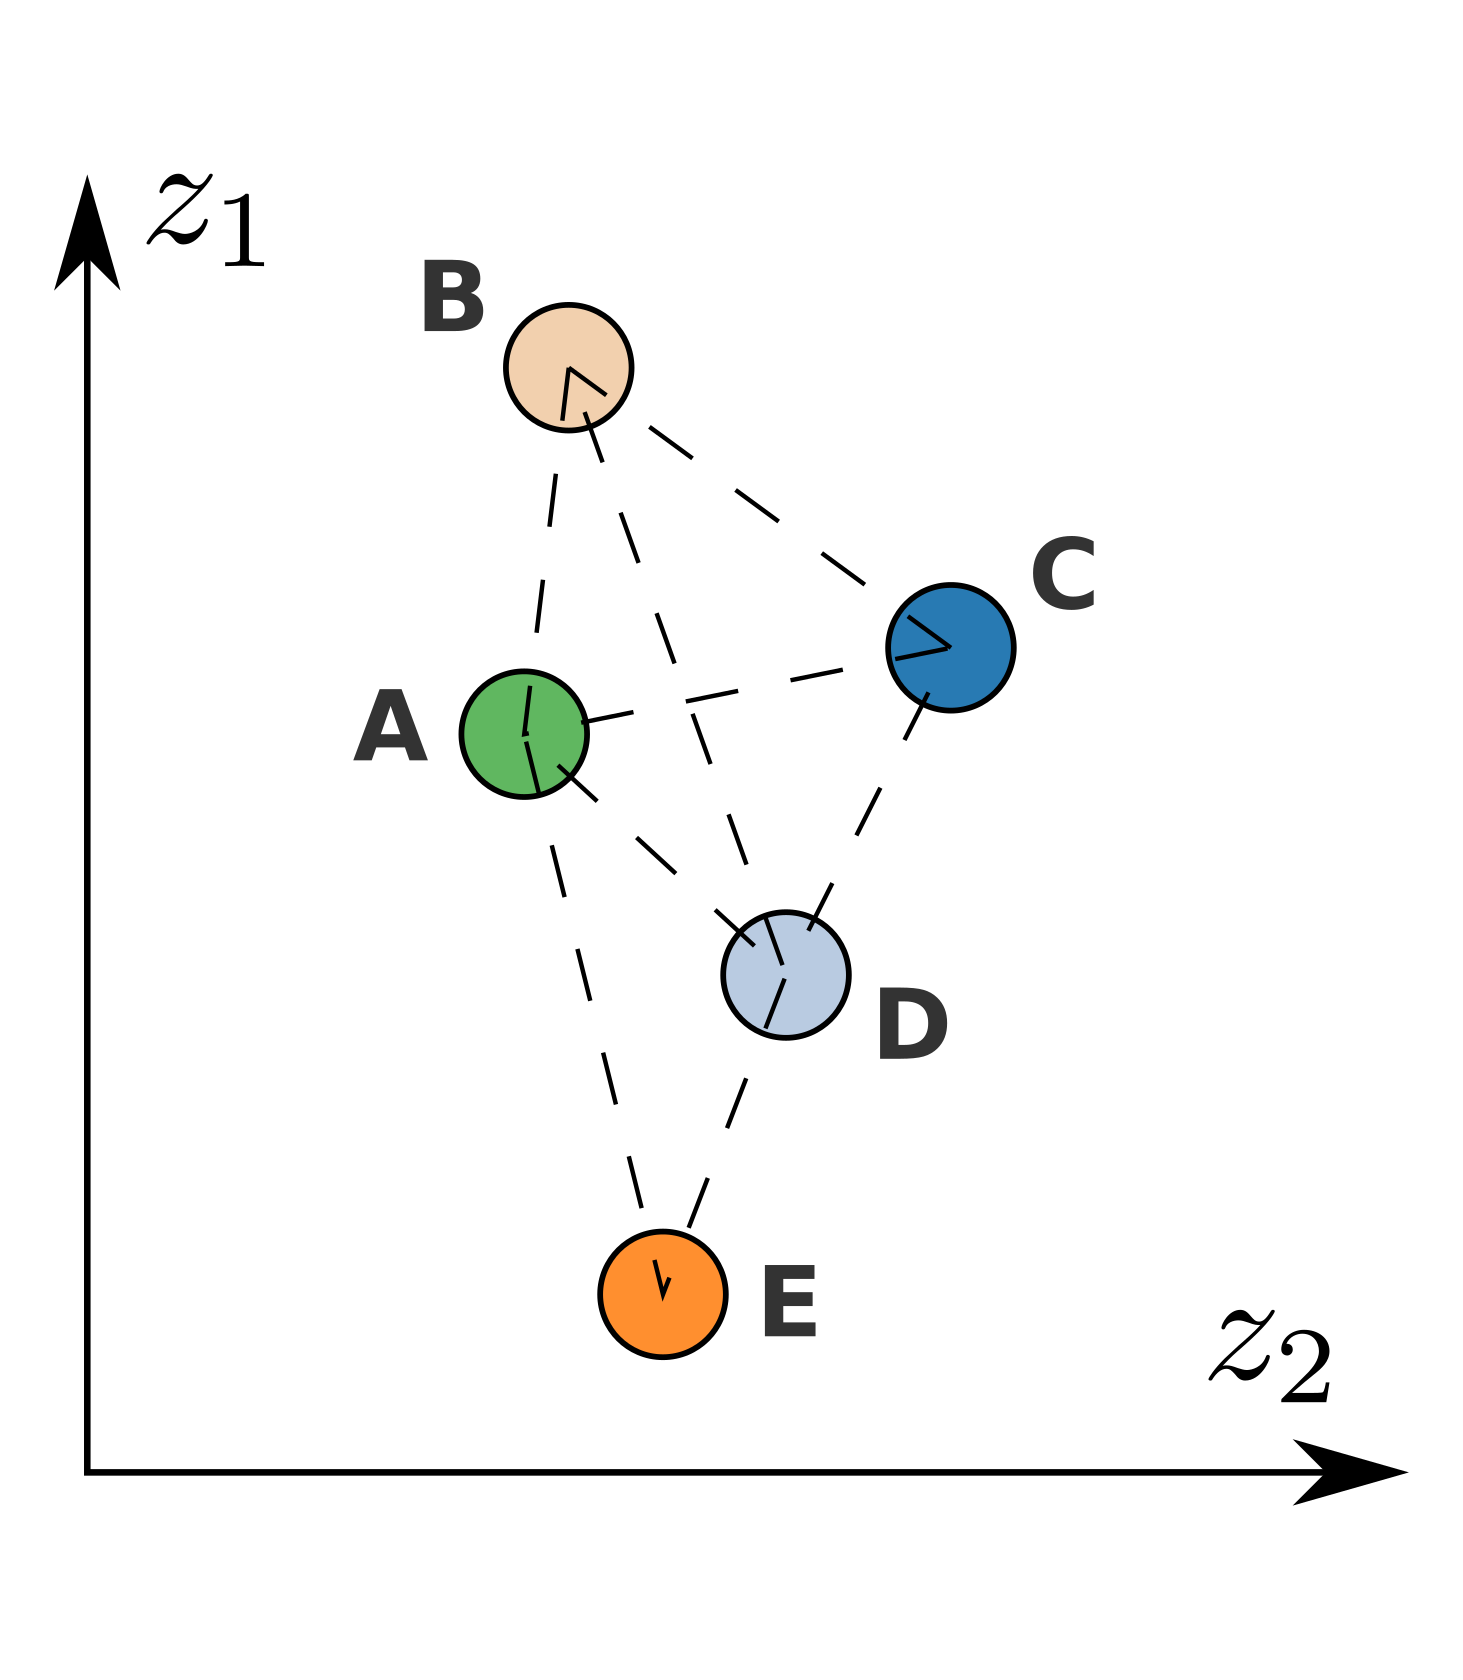
\includegraphics[height=4.5cm]{img/STEP1/voronoi_sketch_2d.png} \label{fig:voronoi_2d}}
    \subfigure{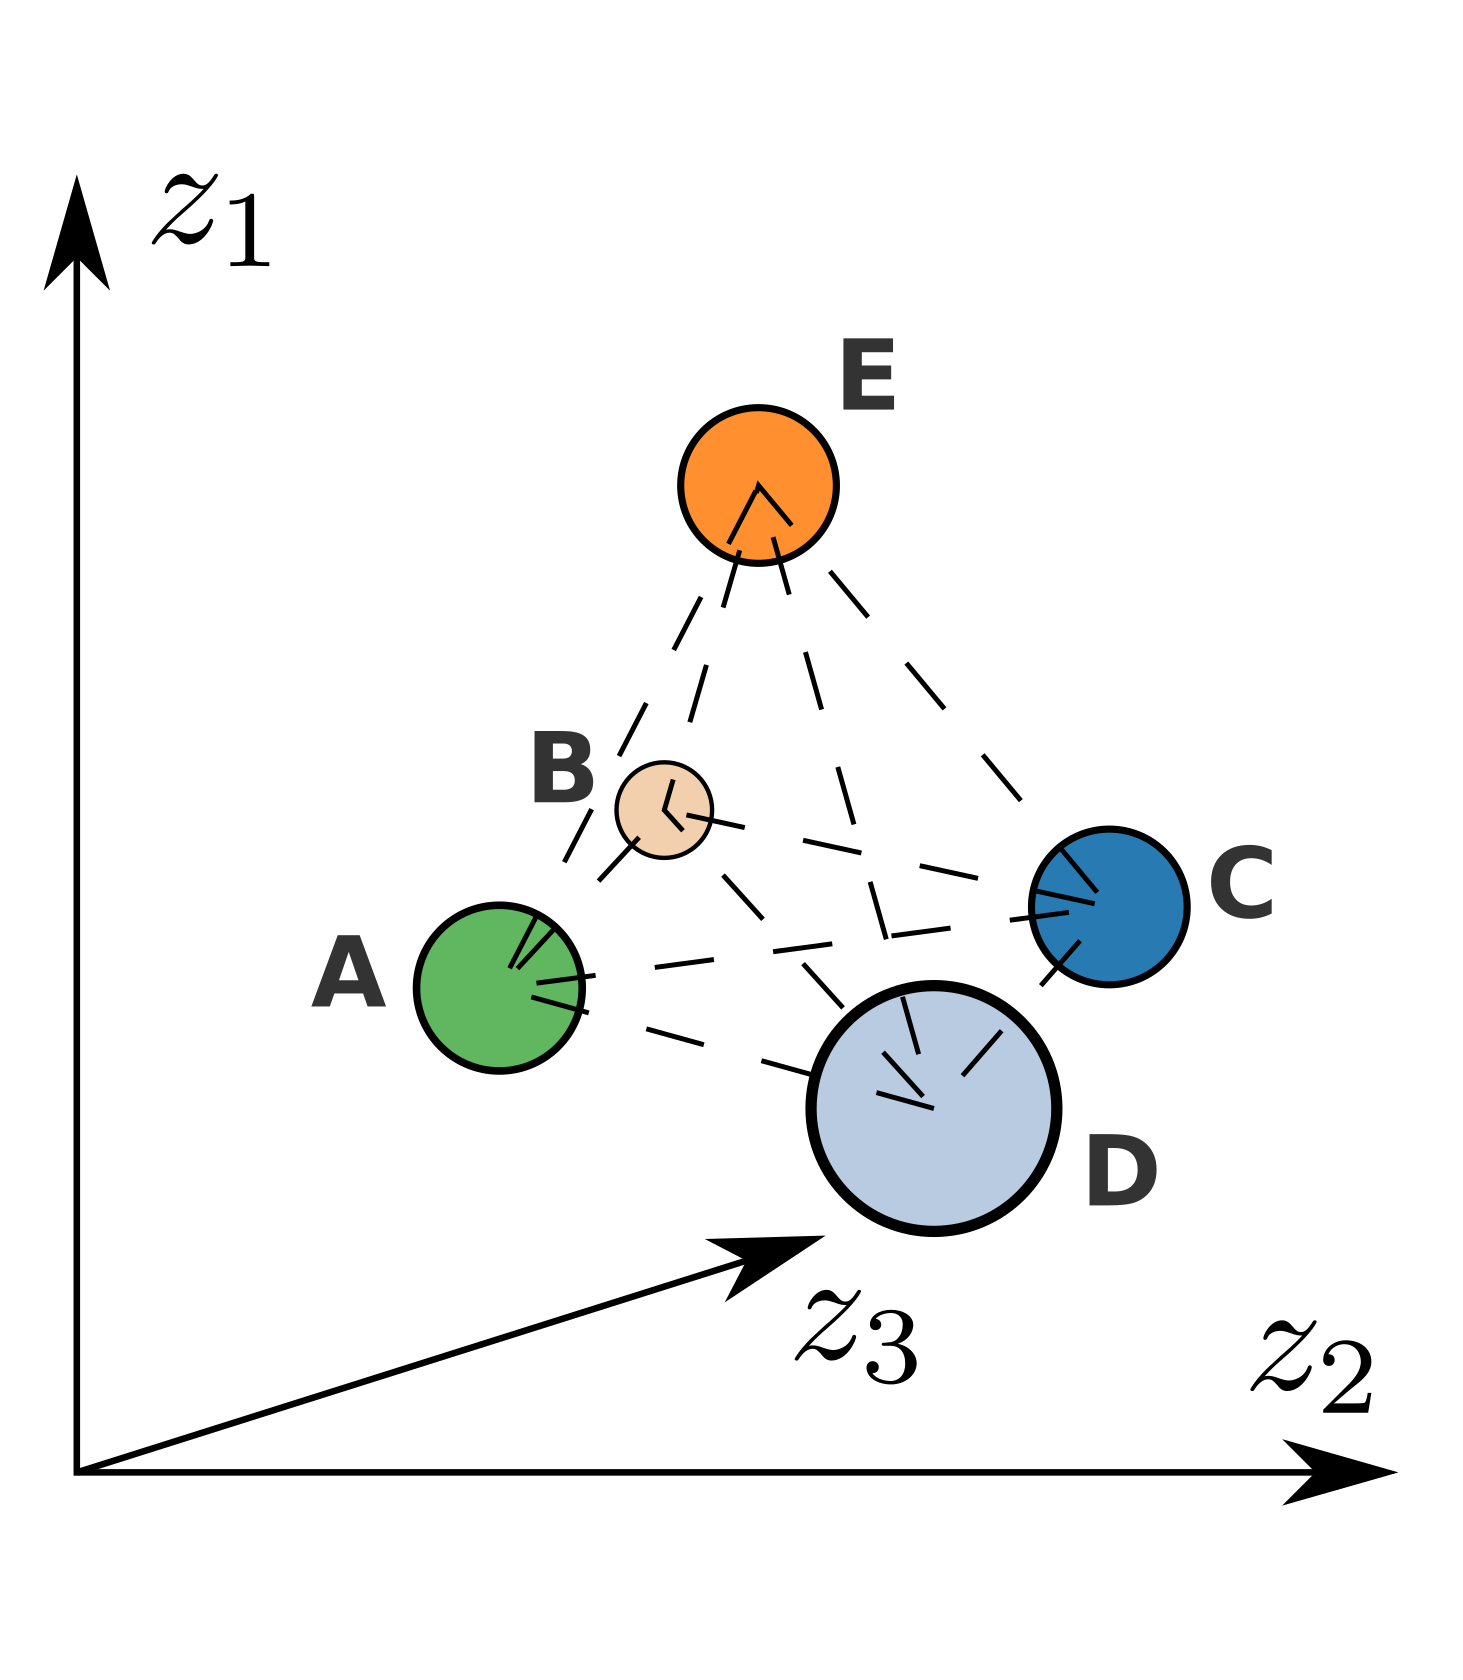
\includegraphics[height=4.5cm]{img/STEP1/voronoi_sketch_3d.png} \label{fig:voronoi_3d}}
    \caption{Topology configurations that is automatically generated upon the training of autoencoder } 
    \label{fig:voronoi}
\end{figure}

\subsection{elastic fitting}
Even if the representation of \VAE{2} seems to present limitations on some class transition, it is although providing a good fitting for the classes in the proposed example as already shown for three instances in~\Figure{\ref{fig:step_1}}. But what has not been shown yet is that there actually is a further subtle structure of the input dataset generator that \VAE{2} captured from covariates. It is another implicit degree of freedom that comes from the fact that we chose to sample along the x-axis from a \textbf{uniform ordered} distribution; this generates samples that are free to span all along the axis but chained with the strict inequality: $\{\bm{x} | x_{i} \geqslant x_{i-1}\}$.
\begin{figure}
    \centering
    \subfigure{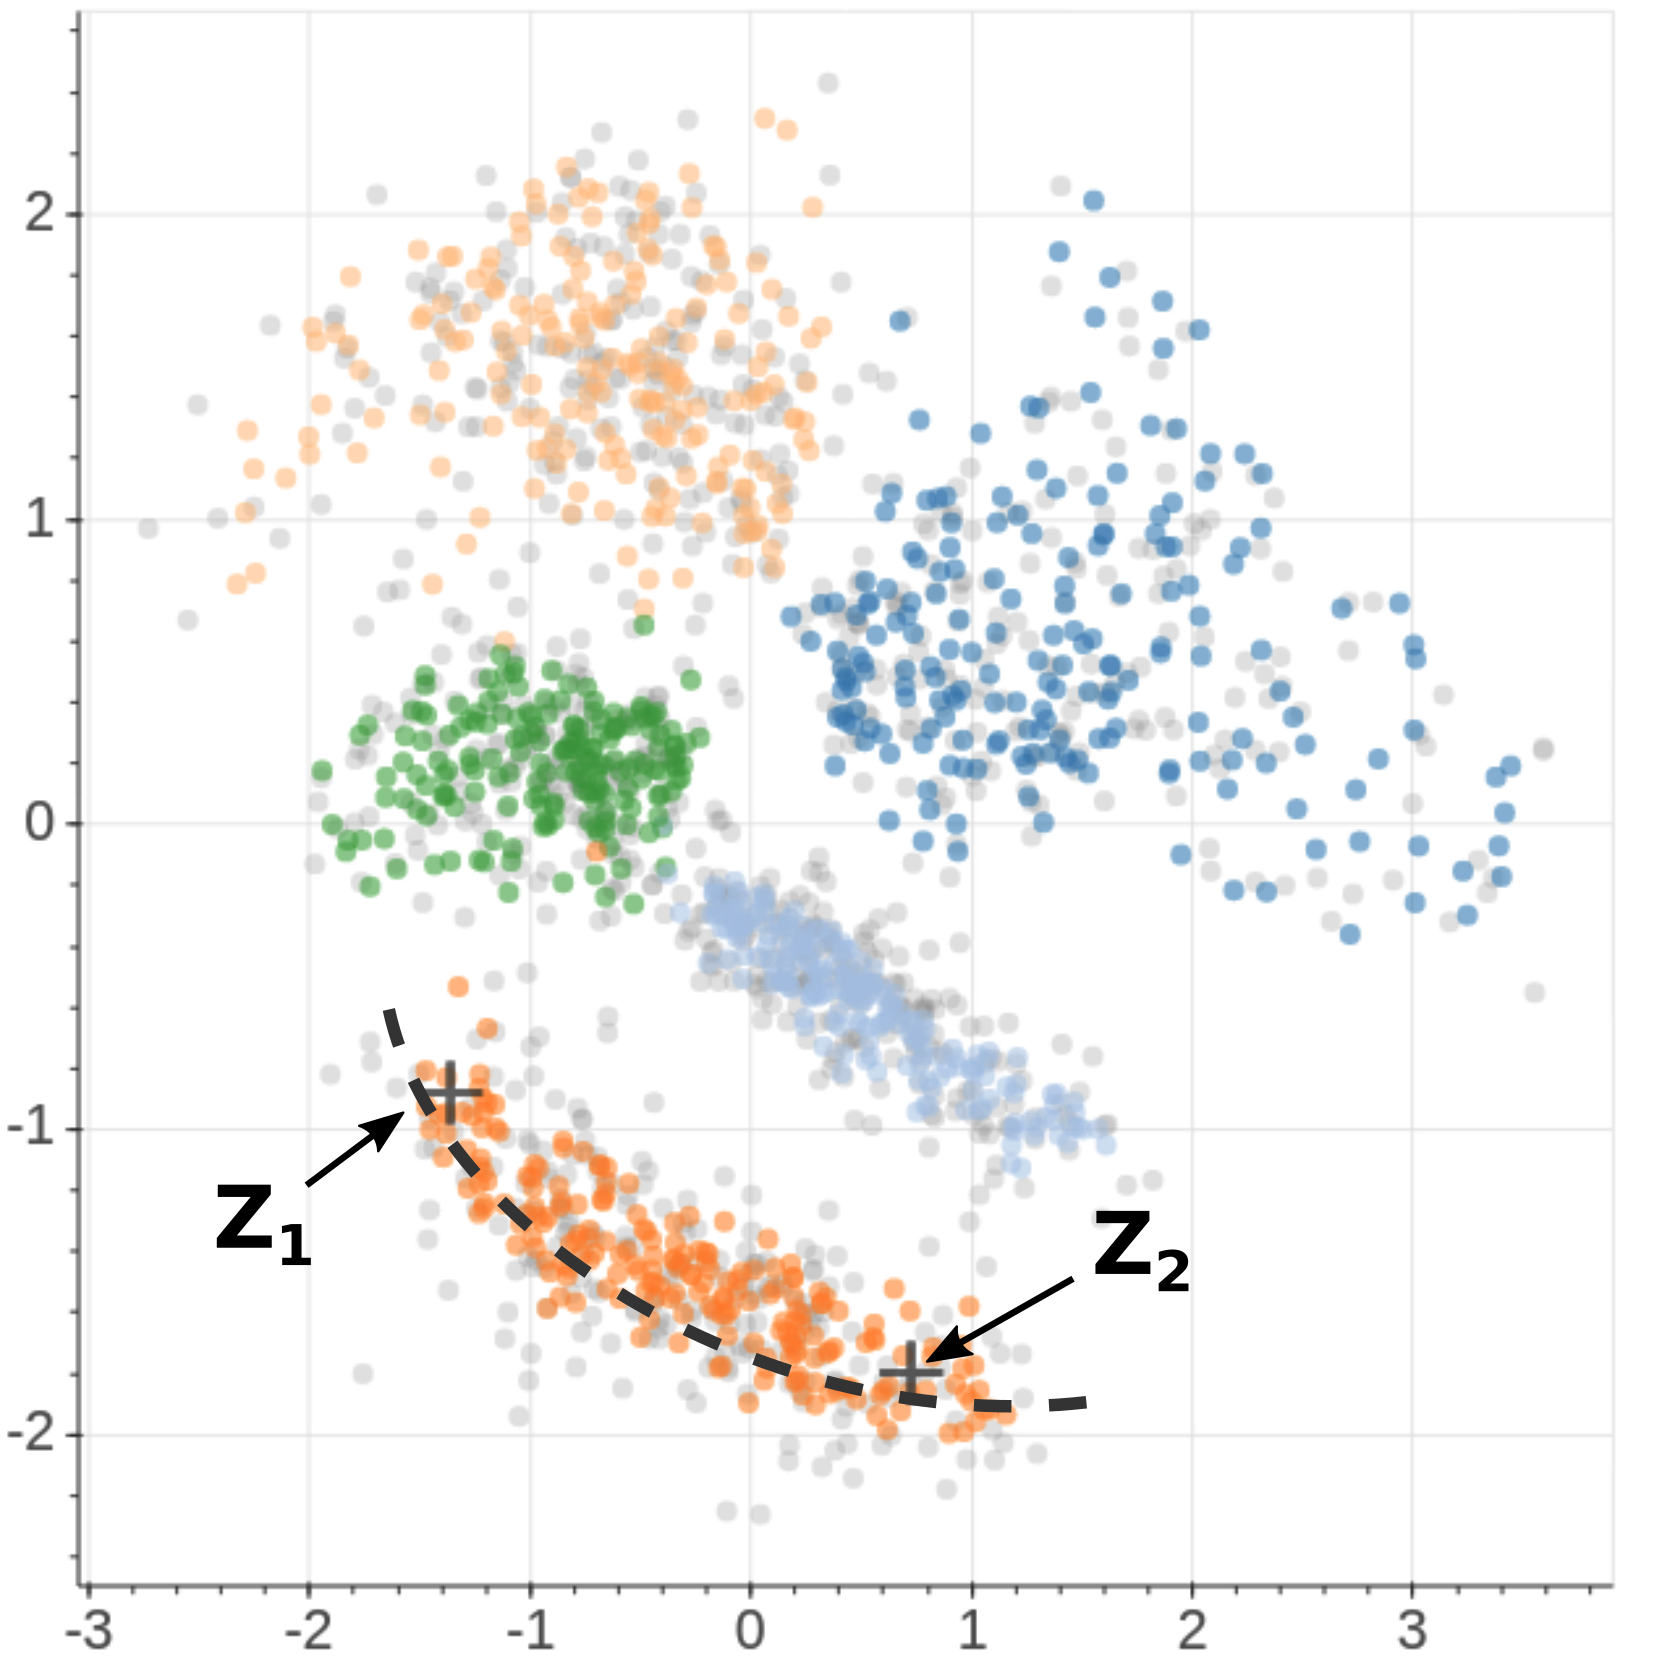
\includegraphics[height=4.5cm]{img/STEP1/elastic_Z1Z2.png} \label{fig:step1_elastic_z1z2}}
    \subfigure{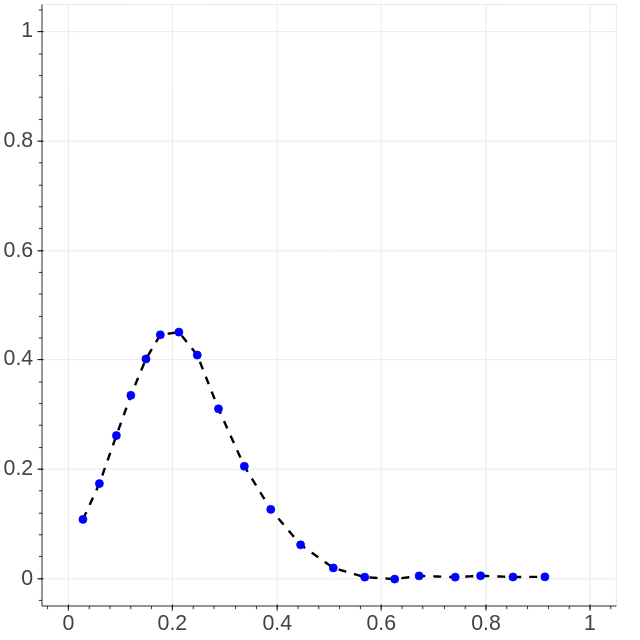
\includegraphics[height=4.5cm]{img/STEP1/elastic_gn1.png}  \label{fig:step1_elastic_gn1}}
    \subfigure{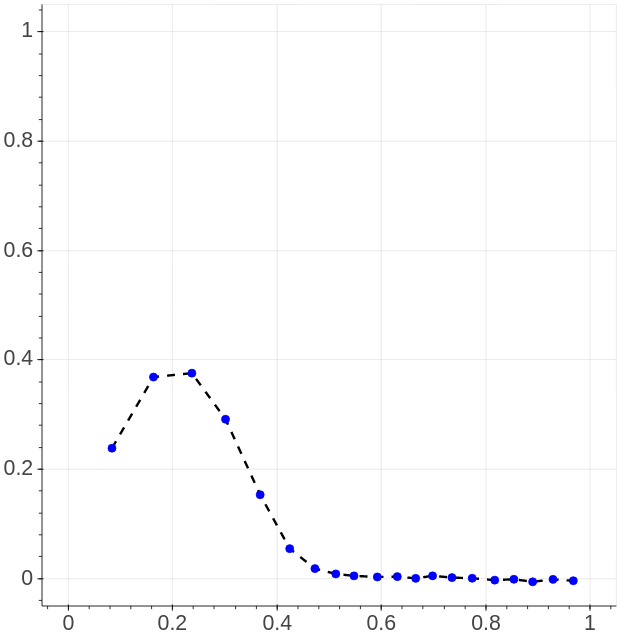
\includegraphics[height=4.5cm]{img/STEP1/elastic_gn2.png}  \label{fig:step1_elastic_gn2}}
    \caption{Elastic latent space reconstruction from \VAE{2} with scatter plot of the latent space and two samples of the same decoded class where it can be seen that the autoencoder distributes the $\bm{x}_1$ positions degree of freedom of the database along the dashed line. Two samples $\bm{z}_1$ and $\bm{z}_2$ have been also plotted from the decoder output to see the elastic effect of the curve points distribution. } 
    \label{fig:step1_elastic}
\end{figure}
This further subdivision of the latent space is hidden in the shape of clusters themselves within one elongated direction. A clear example is visible in~\Figure{\ref{fig:step1_elastic}} where two latent variables points have been decoded and plotted in~\Figure{\ref{fig:step1_elastic_gn1}\ref{fig:step1_elastic_gn2}}; the effect of the x-axis dispersion fit is shown by the fact that even if the overall reconstruction of the curve is quite similar for all chosen points the density of points is different along the axis. Moving one way or the other along the cluster generates curves that remains almost steady in y-axis but wobble in the x-axis density elastically adapting at best all possible choice of points that represent the generating Gaussian formula.

\section{Latent space regularization and disentangled representation}
In the previous section~\cref{section:training_regularization} the concept of \textit{regularization} have been introduced for a supervised network training; in this section the some further methods will be discussed applied to the \acs{VAE} and the latent space reconstruction.
%
One of the major challenge for the today machine learning approaches is the fact that the resulting learned task can vary significantly depending on the choice of the data representation, i.e. the structure of the latent space.
It has been suggested that learning a disentangled representation of the generative factors within covariates can be useful for a large variety of tasks and domains~\cite{Bengio_2013}~\cite{ridgeway2016survey}. A complete disentangled representation can be defined as the network configuration where a single latent unit is sensitive to changes in a single generative factor, while being almost uncorrelated with all the others.
For example, a model that implements a deep convolutional \acs{VAE} trained on a dataset of objects images might learn independent latent units that are sensitive to data generative factors, such as: the actual object class, the position, scale, or colour; thus each latent variable acts as a single self sufficient inversion model. And the most important outcome is that in a disentangled representation, knowledge about one factor can be optimally generalized to novel configurations of the others; for example we could impose a new color of given object even if any sample of that colour has been given in the training dataset.
%
A standard way to promote disentanglement is to augment the original \acs{VAE} framework with a single hyper-parameter $beta$ that modulates the learning constraints applied to model~\cite{Higgins2017betaVAELB}. These constraints impose a limit on the capacity of the latent information channel and control the emphasis on learning statistically independent factors. 
In the so called $\beta-\textrm{VAE}$ the optimized loss that leads to the \textit{evidence lower bound} (presented in \cref{section:VAE}) is modified as:
\begin{equation}
    \mathrm{ELBO}_{q(.)}(\beta) = \log p(\bm{x}) - \beta \left[ \KLD{q(\bm{z})}{p(\bm{z}|\bm{x})} \right]
\end{equation}
With $\beta>1$ the model is pushed to learn a more efficient latent representation of data, which is disentangled if the data contains at least some underlying factors of variation that are independent.
%
\begin{figure}
    \centering
    \subfigure{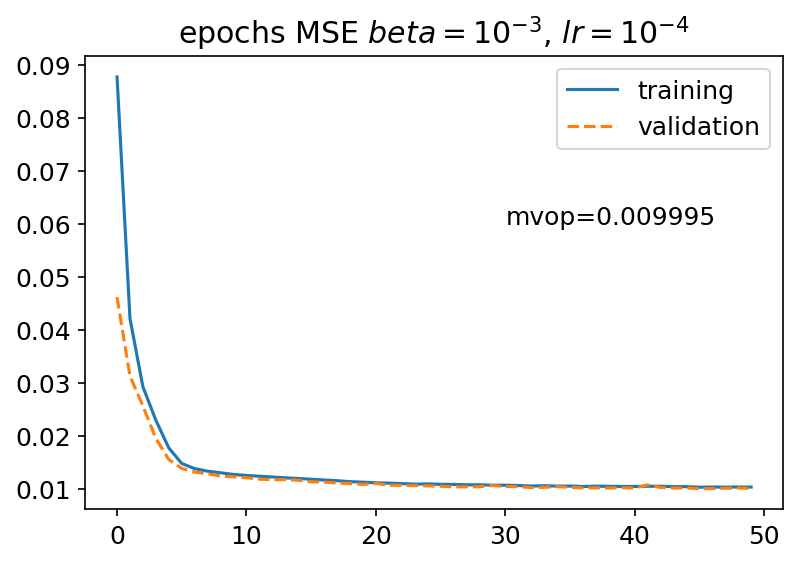
\includegraphics[height=4.5cm]{img/STEP1/training_20-20-10-10_b1e-3.png}    \label{fig:step1_regularization_e3}}
    \subfigure{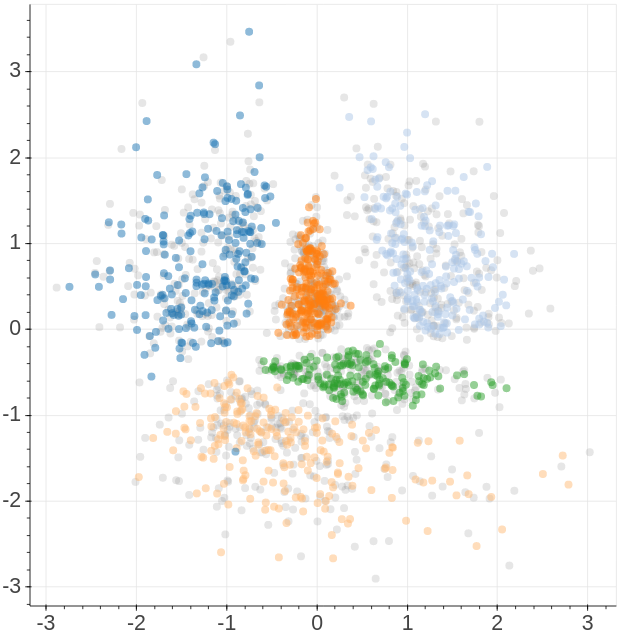
\includegraphics[height=4.5cm]{img/STEP1/training_20-20-10-10_b1e-3_ls.png} \label{fig:step1_regularization_e3_ls}}
    \subfigure{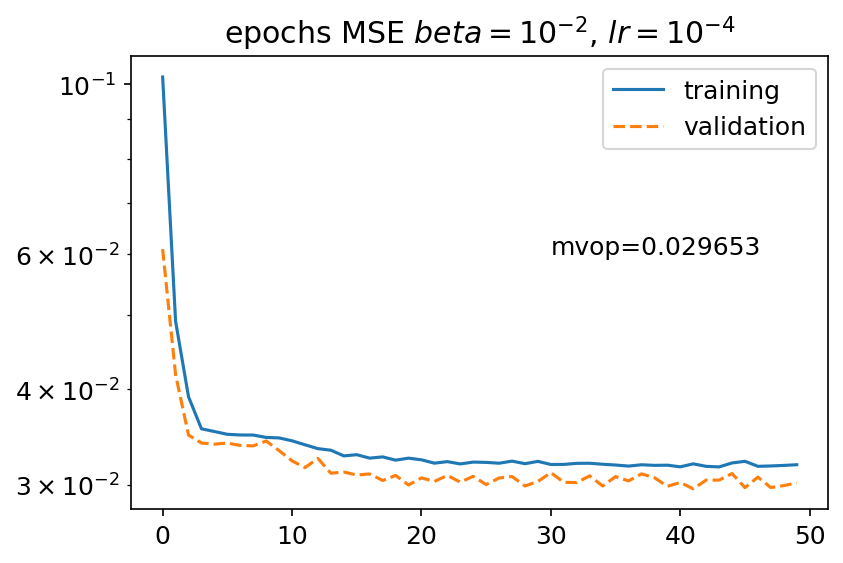
\includegraphics[height=4.5cm]{img/STEP1/training_20-20-10-10_b1e-2_log.png}\label{fig:step1_regularization_e2}}
    \subfigure{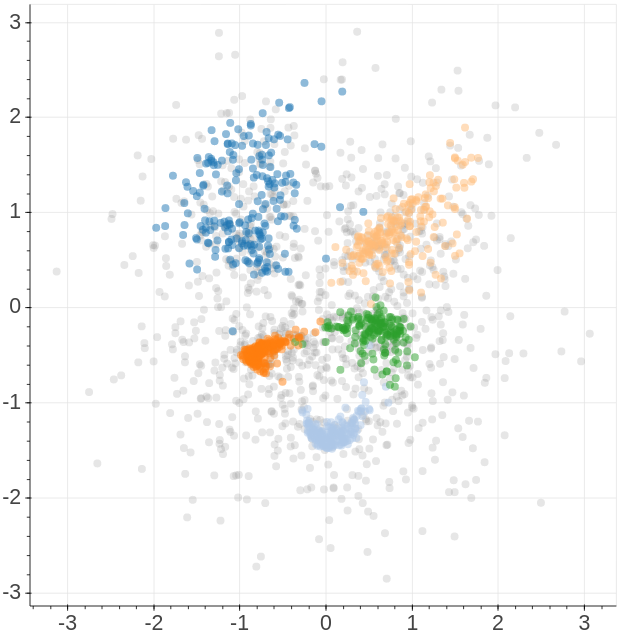
\includegraphics[height=4.5cm]{img/STEP1/training_20-20-10-10_b1e-2_ls.png} \label{fig:step1_regularization_e2_ls}}
    \caption{ Latent space regularization } 
    \label{fig:step1_ls_regularization}
\end{figure}
%
We adopted this solution because it is very easy to be implemented in the \acs{VAE} code being a simple additional loss factor in the KL addendum, and it has been also proved in~\cite{Higgins2017betaVAELB} to produce an effect comparable with other more complex approaches specifically designed for encouraging disentanglement such as InfoGAN~\cite{NIPS2016_6399} or DC-IGN~\cite{kulkarni2015deep}. 
In \Figure{\ref{fig:step1_ls_regularization}} two examples of training from the simulated signals are presented; where the loss per epoch is shown for both the training and validation, and the resulting scattering plot of the latent space for two possible $\beta$ selections.
Seen by the latent space the effect of disentangling factors reflects to a more compact clusters representation. While from the topological point of view the graph of dual Voronoi diagram representation assumes a structure with edges that tend to align with the plot axes, meaning that a single variable is more capable to discriminate the generator classes.
However this comes with a price that is spent by the generator that loose precision in data reconstruction.

\subsection{Noise rejection}
Beside all possible refinements that can be added and are targeted to a better understanding of the latent space, \acs{VAE} can be considered also a robust solution to handle noisy or missing data. Indeed the sole activation of a portion of the network in case of missing covariates, and the recovering of feature from added noise is an outstanding result of the autoencoder. In \Figure{\ref{fig:step1_noise_rejection}} a successful example of both missing data and noise recovery is shown for an instance of the class $k_3$ of the example in \cref{section: gaussian sum generator}. The plot on the left shows with blue ($\bullet$) and dashed curve an instance of the generator, while the orange ($\times$) are the same set where missing values and noise have been applied. From the original set half of measures have been removed and a Gaussian noise with $\sigma=3\times10^{-2}$ has been added. The green line with ($+$) is the resulting decoder output form a \VAE{2}, and it can be seen that it matches the original signal. On the right of the same figure the latent space is plotted for several samples in grey, and a blue dot identify the position of the original curve in latent coordinates, while the orange is the position of the reconstructed one, showing the fit error in latent space.
\begin{figure}
    \centering
    \subfigure[]{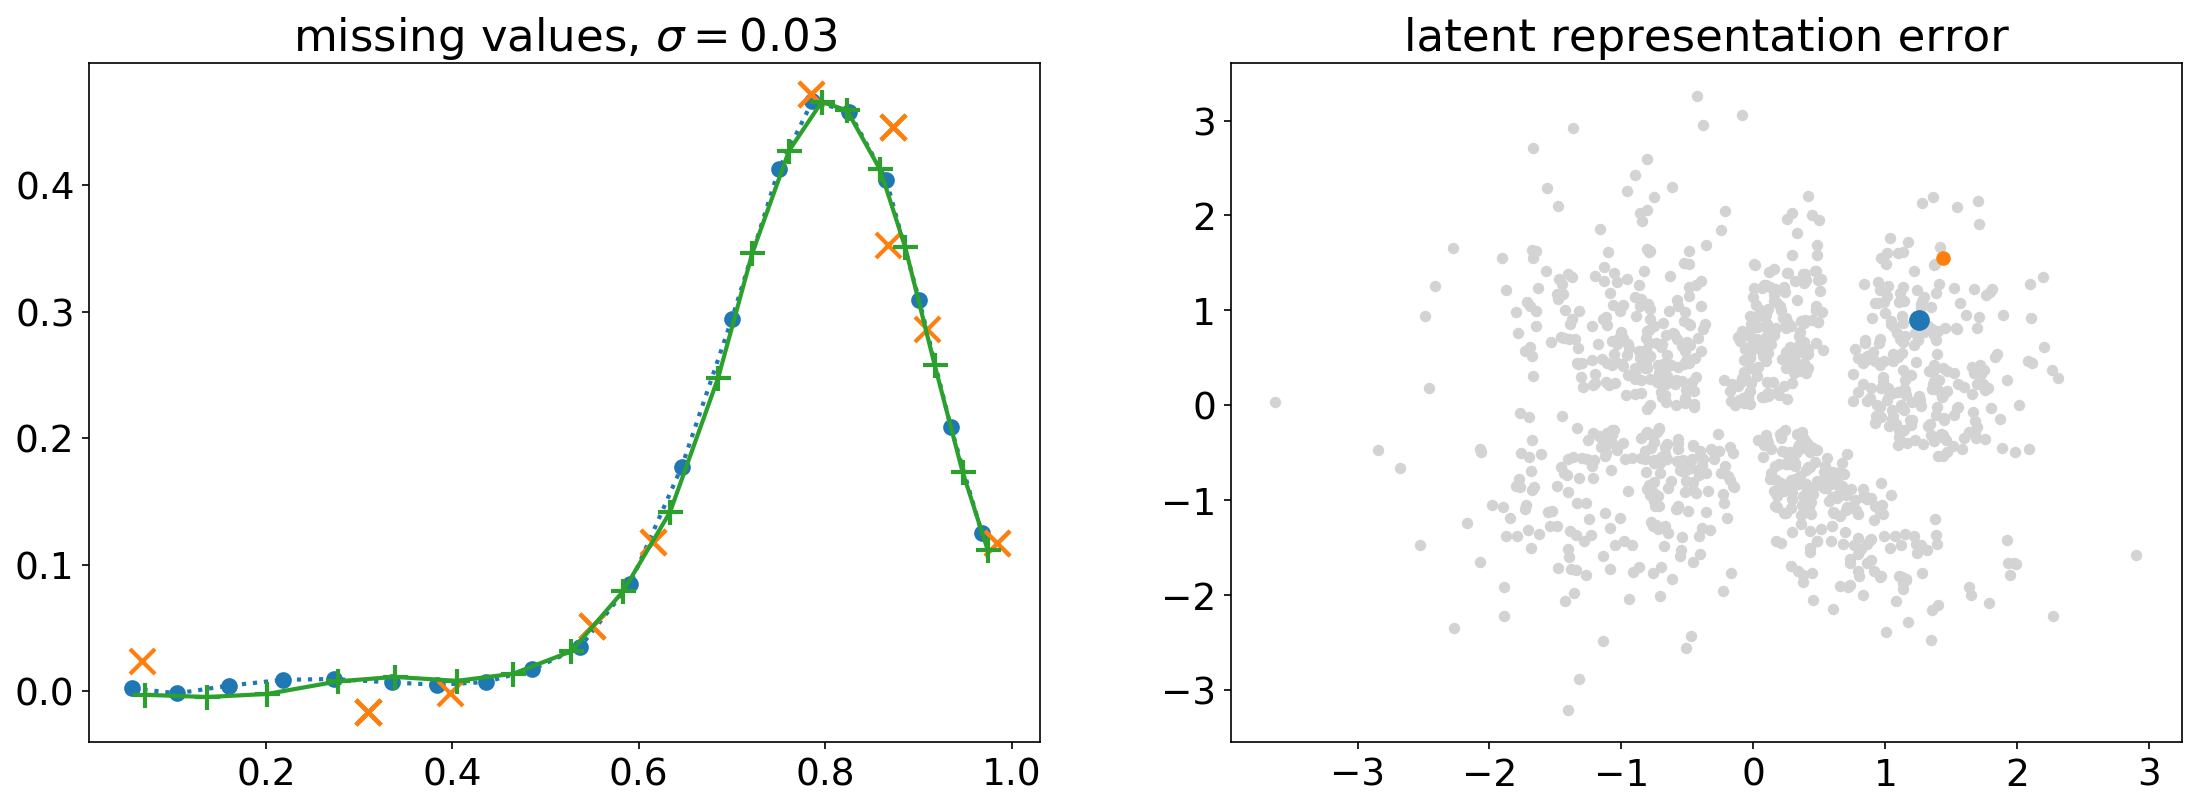
\includegraphics[height=4.5cm]{img/STEP1/recover_noise_err1.png} \label{fig:step1_noise_rejection}}
    \subfigure[]{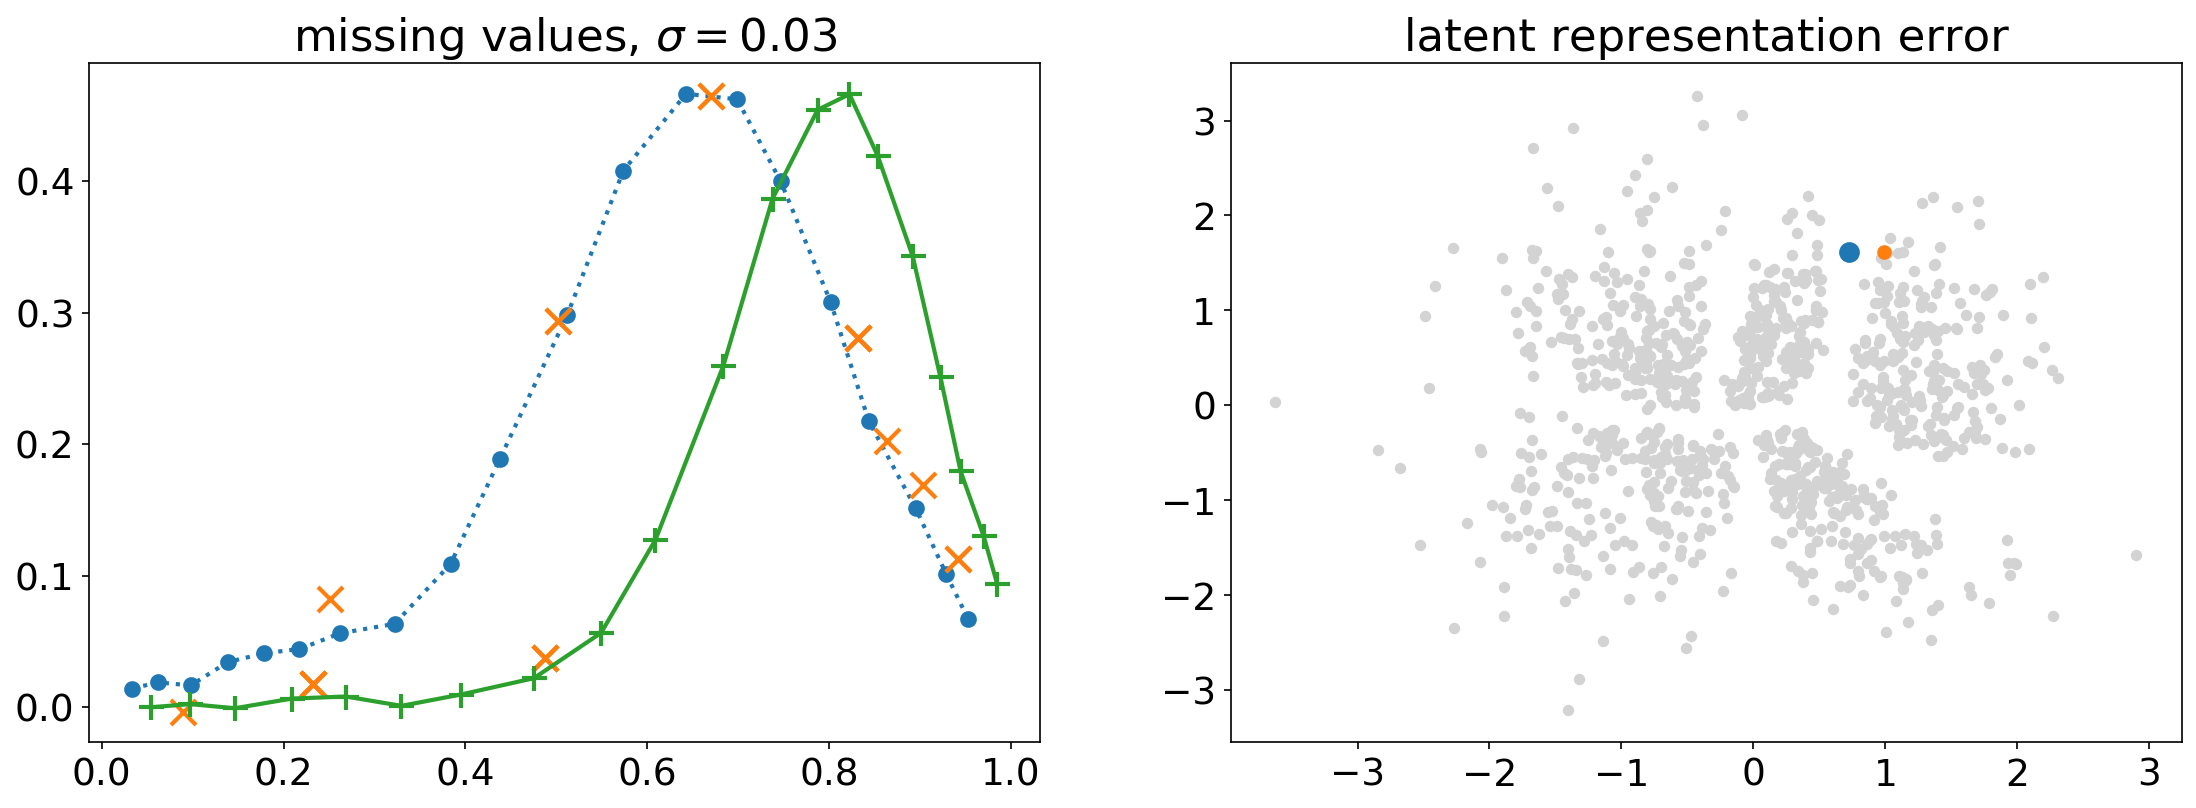
\includegraphics[height=4.5cm]{img/STEP1/recover_noise_err2.png} \label{fig:step1_noise_rejection_failed}}
    \caption{ Noise rejection } 
    \label{fig:step1_noise}
\end{figure}
Although the fitting behavior of the simple \VAE{2} model seems to provide an impressive precision in noise rejection, in this case a careful evaluation on the produced output should be also considered. A clear example is a failed reconstruction from noisy data shown in \Figure{\ref{fig:step1_noise_rejection_failed}}: in this example a curve has been created by the generative network itself by selecting a specific point in the boundary between two classes, to have a critical set of covariates that are not in the training dataset. Than the same noise and missing values of the previous example have been applied as it were a normal input. \VAE{2} in this case applies a recovery of the noise preferring to match a curve that matches a small amount of input data (i.e. the tree orange crosses on the lower right) because those noisy values are compatible with a specific class of curves so it is more likely to be in the original training dataset.


\section{Other Kinds of Networks}

\subsection{Generative Adversarial Networks}

Like the previously described Autoencoders The Generative Adversarial Networks belong to the generative models family. It means that they are able to produce / to generate (we’ll see how) new content. To illustrate this notion of “generative models”, we can take a look at some well known examples of results obtained with GANs.

\subsection{Recurrent Neural Networks}
The defined network topology called \acl{RNN} is ultimately an order dependent network regulariztion of the basic percptron. The vanilla \acs{MLP} takes its inputs in a fixed size vector that restricts the analysis to the finite size ergodic signal. On the other hand the \acs{RNN} are a topology extension that exposes to the input features the network internal state, giving a chance for the model to interpret non-ergodic input windows, and with no predetermined limit in size. \acs{RNN}s take one or many input vectors and produce one or many output vectors in which the output is conditioned not only by direct inputs response, but also by a \textit{hidden state} that represents the current context where input is evolving. In this way, the same input could produce different outputs depending on internal states, and in turn on the previous seen input. Although, this orered sequence of the input covariates is not necessarially time depenent, for example the recurrency could be defined to implement the context analysis of a text.
%
% RR
For supervised learning in discrete time settings, sequences of real-valued input vectors arrive at the input nodes, one vector at a time. At any given time step, each non-input unit computes its current activation (result) as a nonlinear function of the weighted sum of the activations of all units that connect to it. Supervisor-given target activations can be supplied for some output units at certain time steps. For example, if the input sequence is a speech signal corresponding to a spoken digit, the final target output at the end of the sequence may be a label classifying the digit.

An \textit{Elman network} is a three-layer perceptron with the addition of a set of \textit{context} units. The middle (hidden) layer is connected to these context units fixed with a unitary weight. At each step the input is fed forward and the fixed back-ward connections save the previous values of the hidden units in the context ones. In this way the network maintains its inner state:
\begin{align}
    & \bm{x}_t = \sigma_x\left( A\bm{x}_{t-1} + B\bm{u}_t + \bm{w}_t \right) \\
    & \bm{y}_t = \sigma_y\left( C\bm{x}_t + \bm{v}_t \right)
    \label{eq:elman_model}
\end{align}
Similarly the output signal can be used as the inner state as well, in this case the topology structure is referred as the \textit{Jordan} recurrent network:
\begin{align}
    & \bm{x}_t = \sigma_x\left( A\bm{y}_{t-1} + B\bm{u}_t + \bm{w}_t \right) \\
    & \bm{y}_t = \sigma_y\left( C\bm{x}_t + \bm{v}_t \right)
    \label{eq:jordan_model}
\end{align}

%% LSTM %%





% \section{Constraining regularizer with semi-supervised training}























